\documentclass[a4paper]{article}
\usepackage{minted}

\usepackage{polski}
\usepackage[utf8]{inputenc}

\usepackage[export]{adjustbox}
\usepackage{scrextend}
\usepackage{amsfonts}
\usepackage{amsmath}


\usepackage{geometry}
\geometry{a4paper, left=15mm, top=30mm, right=15mm, bottom=20mm}

\usepackage{gensymb}
\usepackage{graphicx} 
\usepackage{isotope}
\usepackage{array}
\usepackage{float}
\usepackage{titlesec}
\usepackage{fancyhdr}
\usepackage{multirow}

\usepackage{hyperref}
\usepackage{sectsty}
\usepackage{enumitem}
\usepackage{listings}
\usepackage[labelformat=simple]{subcaption}
\usepackage{xcolor,colortbl}


\usepackage{tikz}
\usetikzlibrary{shapes.geometric, arrows}
\tikzstyle{startstop} = [
    rectangle, 
    rounded corners, 
    minimum width=3cm, minimum height=1cm,
    text centered,
    draw=black, fill=red!30]
\tikzstyle{io} = [
    trapezium, trapezium left angle=70, trapezium right angle=110, 
    minimum width=3cm, minimum height=1cm, 
    text centered, 
    draw=black, fill=blue!30]
\tikzstyle{process} = [
    rectangle, 
    minimum width=3cm, minimum height=1cm, 
    text centered, 
    draw=black, fill=orange!30]
\tikzstyle{decision} = [
    diamond, 
    minimum width=3cm, minimum height=1cm, 
    text centered, 
    draw=black, fill=green!30]
\tikzstyle{arrow} = [thick,->,>=stealth]

\usepackage{karnaugh-map}

\sectionfont{\normalfont\huge\sectionrule{0pt}{0pt}{-6pt}{1pt}}
\subsectionfont{\normalfont\LARGE}
\subsubsectionfont{\normalfont\Large}

\pagestyle{fancy}
\fancyhf{}
\fancyhead[LE,LO]{\Large Łukasz Kwinta, Kacper Kozubowski, Ida Ciepiela}
\fancyhead[LE,RO]{\Large Układ odliczający}
\fancyfoot[CE,CO]{\Large\thepage}

\renewcommand{\footrulewidth}{1pt}
\renewcommand{\headrulewidth}{1pt}

\definecolor{Gray}{gray}{0.85}
\definecolor{LightGray}{gray}{0.95}

\newcolumntype{a}{>{\columncolor{Gray}}c}
\newcolumntype{b}{>{\columncolor{white}}c}

\hypersetup{
    colorlinks,
    citecolor=black,
    filecolor=black,
    linkcolor=black,
    urlcolor=black
}

\counterwithin{table}{section}
\counterwithin{figure}{section}

\title{\fontsize{30pt}{30pt}\selectfont Laboratorium 2 \\ Układ odliczający}
\author{\fontsize{20pt}{20pt}\selectfont Łukasz Kwinta, Kacper Kozubowski, Ida Ciepiela}
\date{kwiecień 2024}

\begin{document}
\maketitle
\pagebreak
\large
\tableofcontents

\pagebreak
\section{Cel zadania}
\Large
Korzystając wyłącznie z wybranych przerzutników oraz dowolnych bramek logicznych, proszę zaprojektować czterobitowy układ TIMER, odmierzający ustawiany za pomocą przełączników czas (od 0 do 15).
\\\\
Po wciśnięciu przycisku STRAT, układ rozpoczyna odmierzanie czasu do tyłu (proszę dobrać częstotliwość tak, aby efekt był dobrze widoczny na ekranie). 
\\\\
Po wyzerowaniu się licznika czasu, układ powinien się zatrzymać i włączyć alarm świetlny wykorzystujący diodę LED. Po ponownym wciśnięciu przycisku START, 
układ powinien wyłączyć alarm i ponownie rozpocząć odmierzanie ustawionego na przełącznikach czasu.
Aktualny wskazywany przez układ czas proszę pokazywać na wyświetlaczach siedmiosegmentowych.

\section{Idea rozwiązania}
Do rozwiązania zadania wybraliśmy przerzutniki T - z powodu łatwości sterowania takim układem. Do sterowania przerzutnikami
w trybie synchronicznym wykorzystaliśmy transkoder uruchamiający wejścia T kolejnych przerzutników na bazie obecnego 
stanu wyjścia układu. Dodatkowo dodaliśmy pojedynczy sygnał kontrolujący włączenie/wyłączenie układu.

Do początkowego zaprogramowania czasu odliczania na liczniku wykorzystaliśmy możliwość asynchronicznego ustawienia przerzutników
w konkretny stan, również tutaj zaprojektowaliśmy transkoder, który porównuje stan przerzutników z wejściem do programowania 
czasu i odpowiednio ustawia układ. 

\pagebreak
\section{Układ timer}
\subsection{Black box}
Pierwszym krokiem w projektowaniu układu było zaprojektowanie czarnej skrzynki i określenie wejść i wyjść 
układu.
\begin{figure}[H]
    \centering
    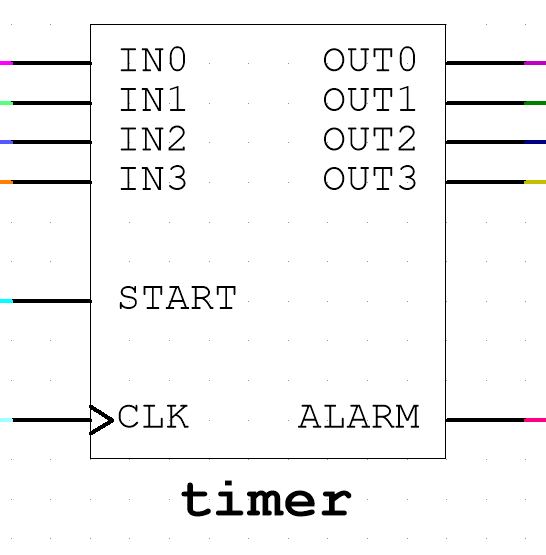
\includegraphics[width=0.4\textwidth]{timer_black_box.png}
    \captionof{figure}{Czarna skrzynka timera}
\end{figure}

Poniżej przedstawimy specyfikację wejść i wyjść układu
\subsubsection{Wejścia}
\begin{itemize}
    \item \verb|INx| - wejścia programujące czas odliczania licznika - binarny zapis liczby od której licznik powinien 
            zacząć odliczać. 4 wejścia łącznie pozwalają na odliczanie w zakresie 0-15. \verb|IN0| oznacza najmniej 
            znaczący bit, \verb|IN3| oznacza najbardziej znaczący bit. Wejście jest używane do zaprogramowania w momencie
            gdy na wejściu \verb|START| pojawi się stan wysoki.
            \begin{center}
                \begin{tabular}{|c|c|c|c|c|}
                  \hline Numer bitu & 3 & 2 & 1 & 0 \\ 
                  \hline Bit & \verb|IN3| & \verb|IN2| & \verb|IN1| & \verb|IN0| \\
                  \hline Mnożnik & $2^3$ & $2^2$ & $2^1$ & $2^0$  \\
                  \hline
                \end{tabular}
                \captionof{table}{Kodowanie pinów wejściowych} 
              \end{center}

    \item \verb|START| - wejście aktywujące układ. Stan wysoki oznacza aktywację licznika, stan niski oznacza, że licznik 
              dokończy liczenie do wyzerowania licznika.

              Jeśli wejście \verb|START| będzie miało stan wysoki w czasie dojścia licznika do zera, na wyjściu \verb|ALARM|
              pojawi się puls, po czym licznik zostanie zaprogramowany obecnym wejściem, a następnie uruchomiony ponownie.
              
              Zmiany stanu na wejściu \verb|START| w czasie gdy licznik jest w stanie liczenia, nie mają żadnego efektu. 

    \item \verb|CLK| - wejście zegara stanowiącego podstawę czasu licznika - określa jak szybko następować będą zmiany wyjścia
              i odliczanie licznika do zera.
\end{itemize}

\subsubsection{Wyjścia}
\begin{itemize}
    \item \verb|OUTx| - wyjścia stanowiące kolejne bity aktualnego stanu licznika. Zmiana wartości licznika, następuje
            na wznoszącym zboczu zegara wejściowego. \verb|OUT0| stanowi najmniej znaczący bit, a \verb|OUT3| najbardziej
            znaczący bit.
            \begin{center}
                \begin{tabular}{|c|c|c|c|c|}
                  \hline Numer bitu & 3 & 2 & 1 & 0 \\ 
                  \hline Bit & \verb|OUT3| & \verb|OUT2| & \verb|OUT1| & \verb|OUT0| \\
                  \hline Mnożnik & $2^3$ & $2^2$ & $2^1$ & $2^0$  \\
                  \hline
                \end{tabular}
                \captionof{table}{Kodowanie pinów wejściowych} 
              \end{center}
              
    \item \verb|ALARM| - wyjście sygnalizujące zakończenie odliczania licznika. Stan wysoki oznacza, że obecny stan licznika
              jest równy 0.

\end{itemize}

\pagebreak
\subsection{Diagram załączania układów}
Poniżej rozpisaliśmy diagram zależności stanu załączenia poszczególnych układów od siebie z którego wynikać będą tabele prawdy.
\small
\begin{center}
    \begin{tikzpicture}[node distance=2cm][H]
        
        \node (if_0) [decision] {Wyjście = 0};
        
        
        \node (if_start_1) [decision, right of=if_0,  xshift=2.5cm] {Start = 1};
        \node (in_start) [io, above of=if_start_1] {Start};

        \node (out_alarm) [io, below of=if_start_1, yshift=-0.5cm] {Alarm};

        \node (en_programming) [process, right of=if_start_1, xshift=2.5cm] {Załącz ustawianie};
        \node (in_time) [io, above of=en_programming] {Czas};

        \node (en_timer) [process, below of=if_0, yshift=-0.5cm] {Załącz kontroler licznika};
        \node (timer) [startstop, below of=en_timer] {Licznik};
        \node (out) [io, below of=timer] {Wyjście};
        
        
        \draw [arrow] (in_start) -- (if_start_1);
        \draw [arrow] (in_time) -- (en_programming);
        
        \draw [arrow] (if_0) -- node[anchor=south] {Tak} (if_start_1);
        \draw [arrow] (if_start_1) -- node[anchor=south] {Tak} (en_programming);
        \draw [arrow] (if_start_1) -- node[anchor=west] {Nie} (out_alarm);

        \draw [arrow] (if_0) -- node[anchor=west] {Nie} (en_timer);

        \draw [arrow] (en_timer) -- node[anchor=west] {Kontrola przerzutników} (timer);
        \draw [arrow] (en_programming) |- node[anchor=north] {Ustawienie przerzutników} (timer);

        \draw[arrow] (timer) -- (out);

        \draw [thick, ->] (out.south) -- ++(0, -1cm) -| node[anchor=north] {Odliczanie}  ++ (-3cm, 0) |- (if_0.west);
    \end{tikzpicture}
    \captionof{figure}{Diagram załączania układów}
\end{center}
\Large

\subsection{Kontrola działania licznika}
Na najwyższym poziomie nasz układ \verb|timer| składa się z dwóch podukładów: \verb|timer_setter| - układu ustawiającego czas odliczania
oraz \verb|timer_driver| układu kontrolującego wejścia T przerzutników. Na tym samym poziomie znajdują się 
przerzutniki stanowiące faktyczny licznik oraz implementacja formuł załączających te układy opisanych tutaj.

Dla czytelności poniżej przyjmujemy następujące oznaczenia:
\begin{itemize}
    \item \verb|EN_SET| - wejście aktywujące w układzie \verb|timer_setter|
    \item \verb|EN_DRV| - wejście aktywujące w układzie \verb|timer_driver|
    \item \verb|EQ0| - wyjście układu \verb|timer_driver| mówiące o tym czy obecny stan licznika to 0 (stan wysoki).
    \item \verb|START| - wejście startowe timera
\end{itemize}

\subsubsection{Tablice prawdy}

Tabela prawdy wynika z schematu kontroli przedstawionego powyżej.
\begin{center}
    \begin{tabular}{|c|c||c|c|}
    \hline \multicolumn{2}{|c||}{Wejście} & \multicolumn{2}{|c|}{Wyjście} \\
    \hline \verb|EQ0| & \verb|START| & \verb|EN_SET| & \verb|EN_DRV| \\
    \hline 0 & 0 & 0 & 1 \\
    \hline 0 & 1 & 0 & 1 \\
    \hline 1 & 0 & 0 & 0 \\
    \hline 1 & 1 & 1 & 0 \\
    \hline 
    \end{tabular}
    \captionof{table}{Tabela prawdy dla stanów aktywacji podukładów} 
\end{center}

\subsubsection{Wyprowadzenie formuł}
Dla wyjścia \verb|EN_SET| możemy odczytać formułę w prost z tabeli:
\[ \verb|EN_SET| = \verb|EQ0| \cdot \verb|START|  \] 
Dla wyjścia \verb|EN_DRV| możemy pokusić się o próbę optymalizacji formuły
przy pomocy tablicy Karnaugh:
\begin{center}
    \begin{karnaugh-map}[2][2][1][$\texttt{START}$][$\texttt{EQ0}$]
      \manualterms{1,1,0,0}
      \implicant{0}{1}
    \end{karnaugh-map}
    \captionof{table}{Tablica Karanugh dla formuły aktywującej układ kontrolujący licznik} 
\end{center}
Możemy z niej odczytać zoptymalizowaną formułę:
\[ \verb|EN_DRV| = \textcolor{red}{\overline{\texttt{EQ0}}} \]

\pagebreak
\subsubsection{Realizacja formuł}
Poniżej przedstawiamy realizację wcześniej wyprowadzonych formuł:
\[ \verb|EN_SET| = \verb|EQ0| \cdot \verb|START|  \] 
\[ \verb|EN_DRV| = \overline{\texttt{EQ0}} \]
\begin{figure}[H]
    \centering
    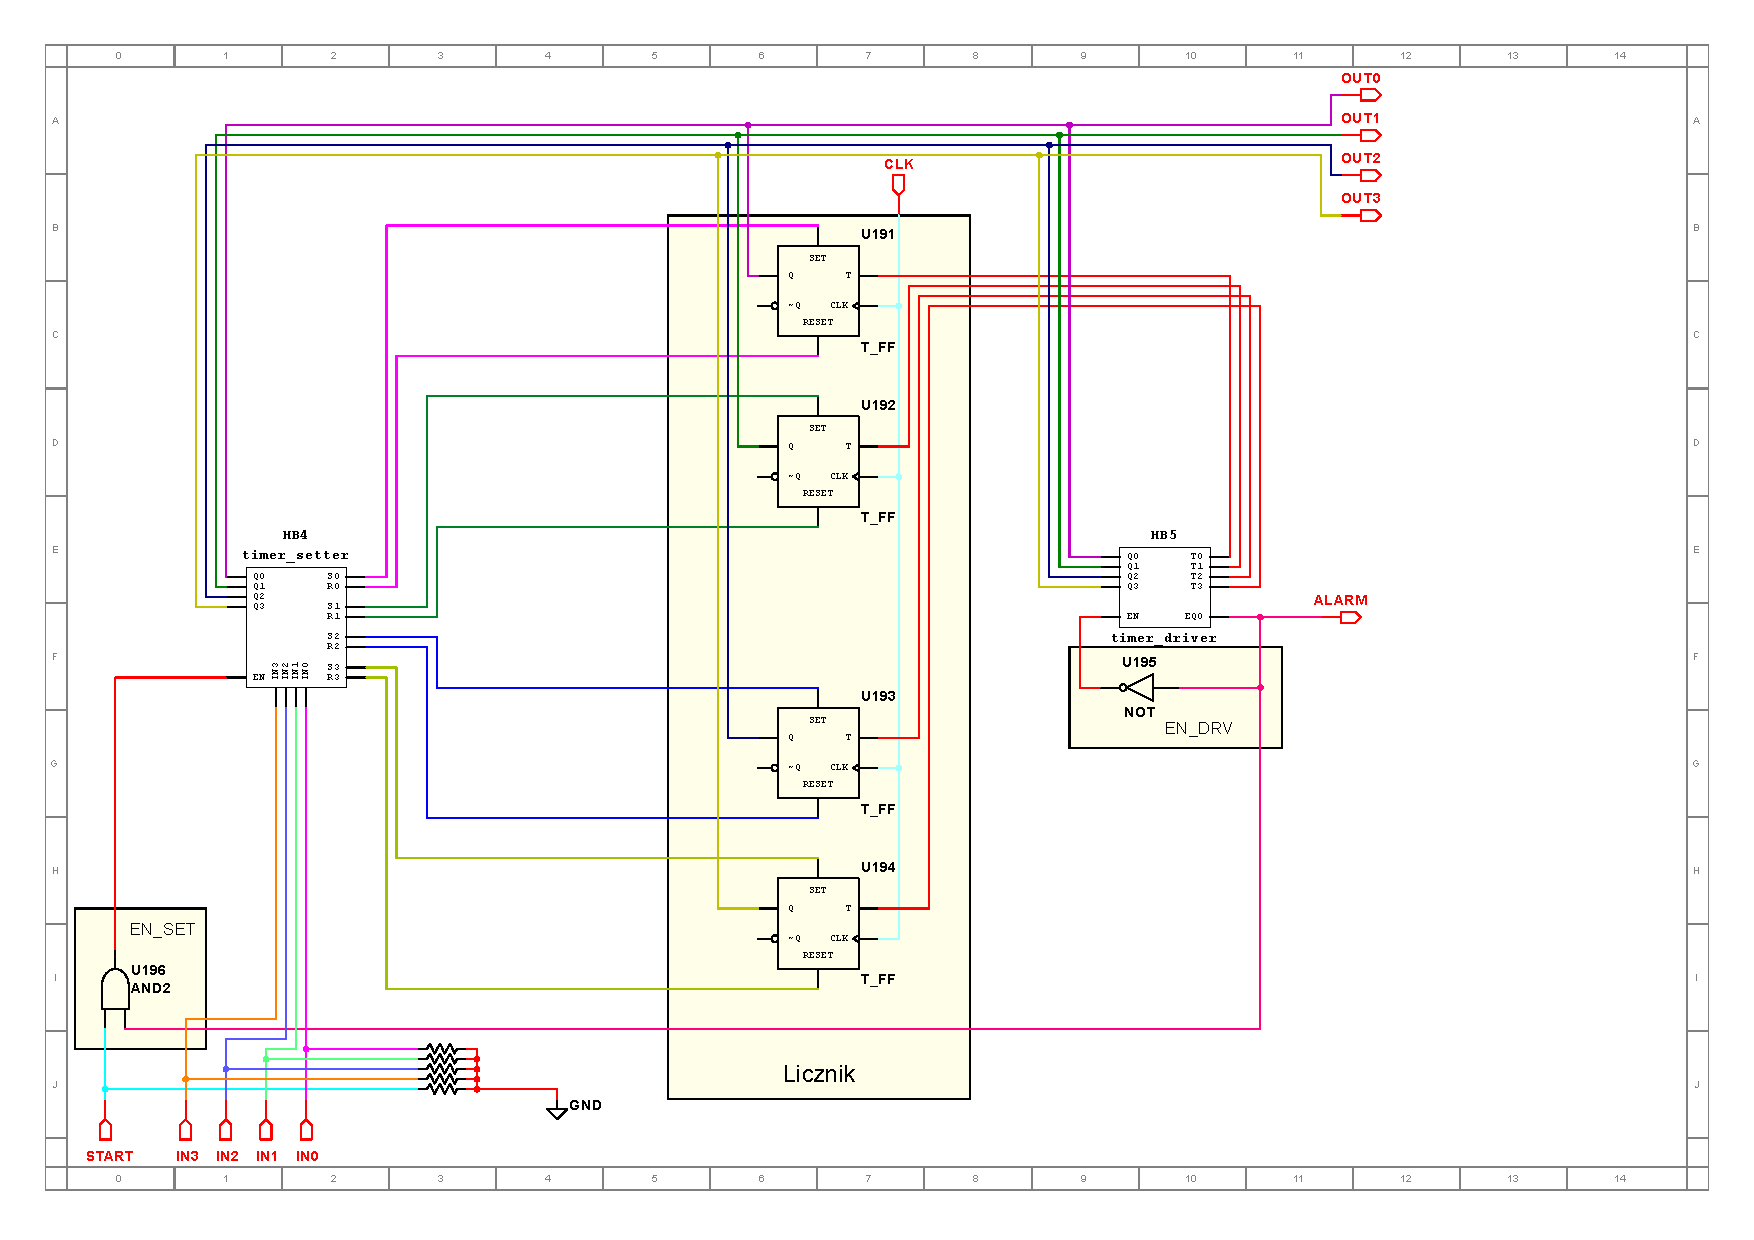
\includegraphics[width=\textwidth]{timer_subsheet.pdf}
    \captionof{figure}{Ogólny schemat timera}
\end{figure}
Na schemacie znajdują się również rezystory pull-down zabezpieczające wejścia układu przed 
nieokreślonym stanem wejść.

\pagebreak
\subsection{Podukład ustawiający czas licznika}
Układ nazwany na naszych schematach \verb|timer_setter| ustawia czas odliczania 
gdy układ zostanie załączony. Układ ma na celu wysterowanie asynchronicznych wejść przerzutników T
poprzez odpowiednie wykonanie operacji SET lub RESET w zależności od obecnego stanu przerzutnika w 
porównaniu do odpowiadającego bitu programowania.

\subsubsection{Wejścia i Wyjścia}
Wejścia do układu stanowią bity oznaczające obecny stan poszczególnych wyjść przerzutnika, bity
oznaczające stan wejścia programowania timera oraz sygnał załączający układ. Wyjścia natomiast 
stanowią pary pinów SET i RESET dla poszczególnych przerzutników. 

\begin{figure}[H]
    \centering
    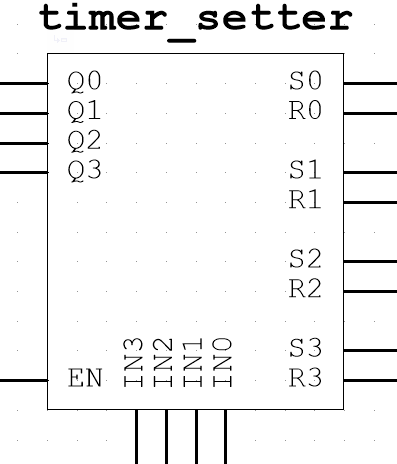
\includegraphics[width=0.4\textwidth]{timer_setter_black_box.png}
    \captionof{figure}{Czarna skrzynka podukładu timer\_setter}
\end{figure}
Poniżej opis wejść układu:
\begin{itemize}
    \item \verb|EN| - wejście aktywujące układ, gdy wejście jest w stanie wysokim, na wyjściach układu
            pojawiają się odpowiednie wartości
    \item \verb|Qx| - wejścia obecnego stanu licznika, \verb|Q0| stanowi najmniej znaczący bit obecnego stanu licznika,
            a \verb|Q3| najbardziej znaczący bit.
    \item \verb|INx| - wejścia programowania startowego stanu licznika, \verb|IN0| stanowi najmniej znaczący bit wejścia,
            a \verb|IN3| najbardziej znaczący bit.
\end{itemize}

Poniżej opis wyjść układu:
\begin{itemize}
    \item \verb|Sx| - wyjście SET ustawiające odpowiedni przerzutnik T, wartość \verb|S0| obliczana
            jest na podstawie wejść \verb|Q0| i \verb|IN0|, a więc odpowiada ustawieniu przerzutnika T
            odpowiadającemu najmniej znaczącemu bitowi licznika.
    \item \verb|Rx| - wyjście RESET resetujący odpowiedni przerzutnik T, wartość \verb|R0| obliczana
            jest na podstawie wejść \verb|Q0| i \verb|IN0|, a więc odpowiada resetowaniu przerzutnika T
            odpowiadającemu najmniej znaczącemu bitowi licznika.
\end{itemize}

\subsubsection{Tabele prawdy}
Jako że, układ oblicza każdą parę wyjść dokładnie tak samo na podstawie odpowiadających sobie bitów,
tabelę prawdy zapiszemy w postaci sparametryzowanej, tzn. parze wyjściowej \verb|Sx|, \verb|Rx| odpowiadają
wejścia \verb|INx|, \verb|Qx| oraz sygnał enable. Finalnie ostateczny układ stanowią 4 powtórzone takie formuły 
dla każdego z bitów 0,1,2,3.

Tabela prawdy wynika z następujących faktów:
\begin{itemize}
    \item jeśli $ \verb|EN| = 0 $ to żadne wyjście nie jest aktywne
    \item jeśli $ \verb|INx| = \verb|Qx| $ to nie musimy zmieniać stanu przerzutnika
    \item w pozostałych przypadków wykonujemy odpowiednio albo operację SET albo RESET
\end{itemize}

\begin{center}
    \begin{tabular}{|c|c|c||c|c|}
    \hline \multicolumn{3}{|c||}{Wejście} & \multicolumn{2}{|c|}{Wyjście} \\
    \hline \verb|EN| & \verb|INx| & \verb|Qx| &  \verb|Sx| & \verb|Rx| \\
    \hline 0 & 0 & 0 & 0 & 0 \\
    \hline 0 & 0 & 1 & 0 & 0 \\
    \hline 0 & 1 & 0 & 0 & 0 \\
    \hline 0 & 1 & 1 & 0 & 0 \\
    \hline 1 & 0 & 0 & 0 & 0 \\
    \hline 1 & 0 & 1 & 0 & 1 \\
    \hline 1 & 1 & 0 & 1 & 0 \\
    \hline 1 & 1 & 1 & 0 & 0 \\
    \hline 
    \end{tabular}
    \captionof{table}{Tabela prawdy dla układu programującego początkowy stan licznika} 
\end{center}

\subsubsection{Wyprowadzenie formuł}
Na podstawie tabeli prawd możemy wyprowadzić formułę na wyjścia \verb|Sx| i \verb|Rx|
\[\verb|Sx| = \verb|EN| \cdot \verb|INx| \cdot \overline{\texttt{Qx}}\]
\[\verb|Rx| = \verb|EN| \cdot \overline{\texttt{INx}} \cdot \texttt{Qx}\]

\subsubsection{Realizacja formuł}
Wyżej wymienione formuły można w multisimie przedstawić w następujący sposób:
\begin{figure}[H]
    \centering
    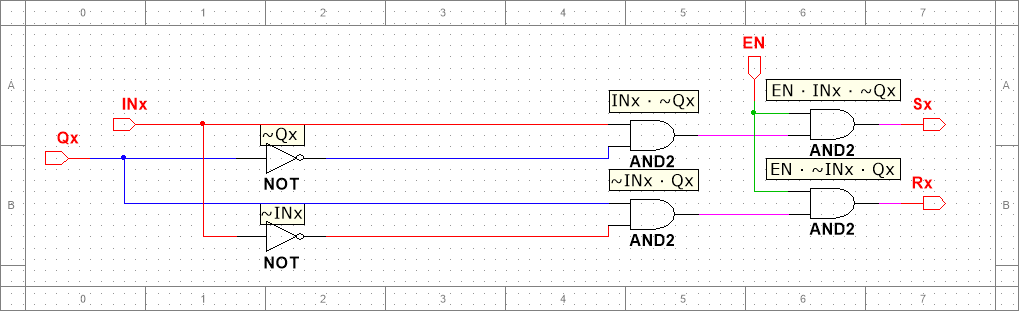
\includegraphics[width=\textwidth]{model1.png}
    \captionof{figure}{Realizacja funkcji logicznych w Multisimie}
\end{figure}
Układ \texttt{timer\_setter} został zaimplementowany jako czterokrotne powielenie powyższej struktury.

\begin{figure}[H]
    \centering
    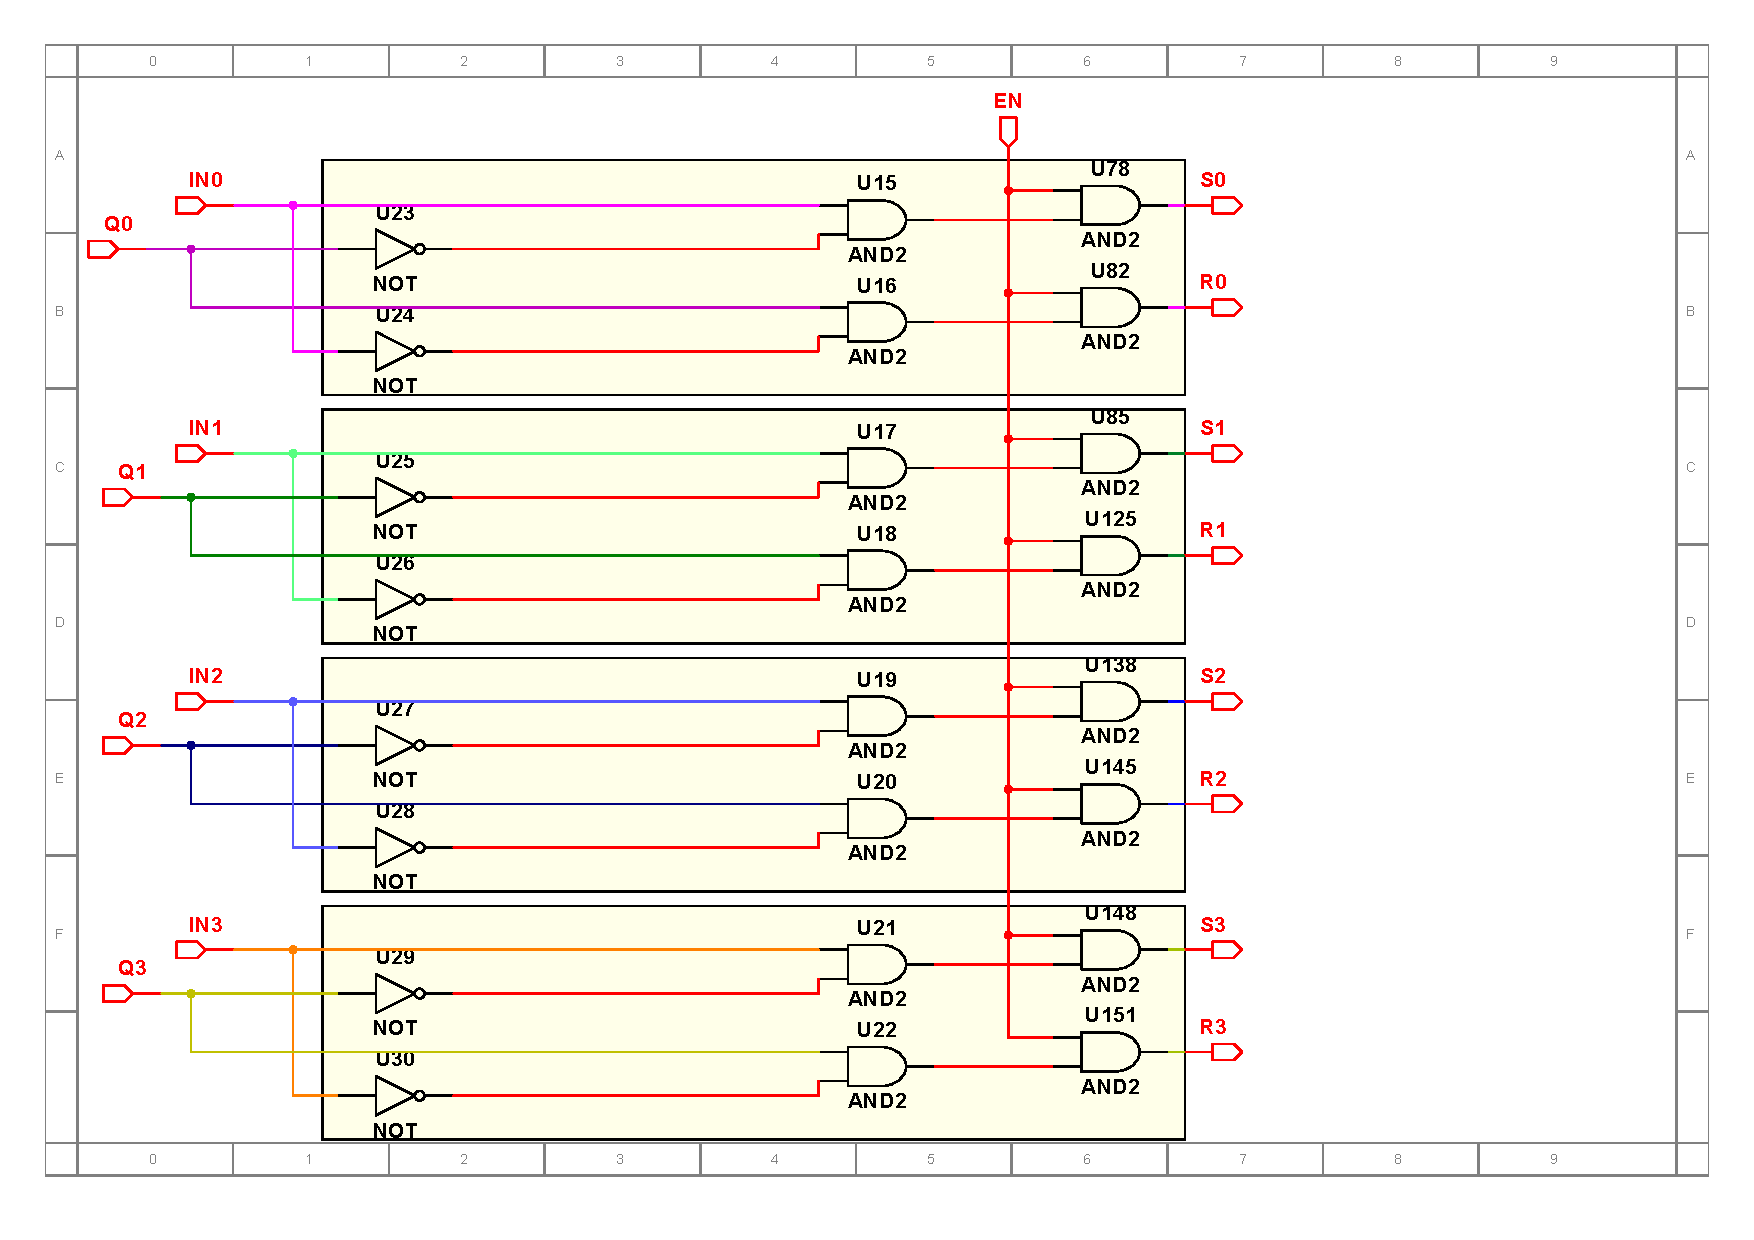
\includegraphics[width=\textwidth]{timer_setter_subsheet.pdf}
    \captionof{figure}{Schemat podukładu: \texttt{timer\_setter}}
\end{figure}

\pagebreak
\subsection{Podukład kontrolujący przerzutniki}
Układ nazwany na naszych schematach \verb|timer_driver| kontroluje wejścia $T$ przerzutników.


\subsubsection{Wejścia i Wyjścia}
Opis wejść układu:
\begin{itemize}
    \item \verb|EN| - Wejście aktywujące układ. Pozwala, aby na wyjściu pojawiały się odpowiednie wartości kiedy jest w stanie wysokim
    \item \verb|Qx| - wejścia obecnego stanu licznika, \verb|Q0| stanowi najmniej znaczący bit obecnego stanu licznika,
            a \verb|Q3| najbardziej znaczący bit.
\end{itemize}

Opis wyjść układu:

\begin{itemize}
    \item \verb|EQ0| - Wyjście informujące o tym czy obecny stan licznika jest równy 0.
    \item \verb|Tx| - wyjścia przerzutnika, \verb|T0| stanowi najmniej znaczący bit przerzutnika,
    a \verb|T3| najbardziej znaczący bit.
\end{itemize}

\begin{figure}[H]
    \centering
    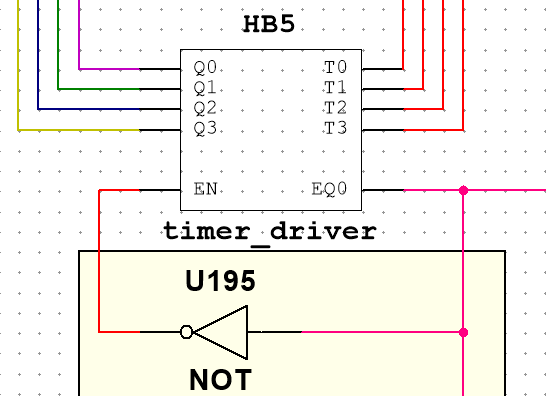
\includegraphics[width=0.5\textwidth]{timer_driver_black_box.png}
    \captionof{figure}{Czarna skrzynka podukładu: \texttt{timer\_driver}}
\end{figure}

\pagebreak
\subsubsection{Tabele prawdy}

Tabela prawdy została skonstruowana na podstawie formuły 
\[T_x =  \verb|XOR|(Q_{n_x},  Q_{n_x+1})\]
gdzie $Q_{n_x}$ oznacza stan obecny, a $Q_{n_x+1}$ oznacza stan następny. Bierze się to z faktu, 
że musimy zmienić stan przerzutnika tylko w momencie kiedy obecny stan nie odpowiada stanowi następnemu
co odpowiada funkcji \verb|XOR|.

\begin{center}
    \begin{tabular}{|l|l|l|l|l||l|l|l|l||l|l|l|l|}
    \hline
    &\multicolumn{4}{c||}{Stan Obecny} & \multicolumn{4}{|c||}{Stan Następny} & \multicolumn{4}{|c|}{Przerzutniki} \\\hline
       &$Q_{n_3}$ & $Q_{n_2}$ & $Q_{n_1}$ & $Q_{n_0}$ & $Q_{n_3+1}$ & $Q_{n_2+1}$ & $Q_{n_1+1}$ &$Q_{n_0+1}$ & $T_3$ & $T_2$ & $T_1$ & $T_0$ \\ \hline
    15 & 1 & 1 & 1 & 1 & 1 & 1 & 1 & 0 & 0 & 0 & 0 & 1 \\ \hline
    14 & 1 & 1 & 1 & 0 & 1 & 1 & 0 & 1 & 0 & 0 & 1 & 1 \\ \hline
    13 & 1 & 1 & 0 & 1 & 1 & 1 & 0 & 0 & 0 & 0 & 0 & 1 \\ \hline
    12 & 1 & 1 & 0 & 0 & 1 & 1 & 0 & 1 & 0 & 1 & 1 & 1 \\ \hline
    11 & 1 & 1 & 0 & 1 & 1 & 0 & 1 & 0 & 0 & 0 & 0 & 1 \\ \hline
    10 & 1 & 0 & 1 & 0 & 1 & 0 & 0 & 1 & 0 & 0 & 1 & 1 \\ \hline
    9  & 1 & 0 & 0 & 1 & 1 & 0 & 0 & 0 & 0 & 0 & 0 & 1 \\ \hline
    8  & 1 & 0 & 0 & 0 & 0 & 1 & 1 & 1 & 1 & 1 & 1 & 1 \\ \hline
    7  & 0 & 1 & 1 & 1 & 0 & 1 & 1 & 0 & 0 & 0 & 0 & 1 \\ \hline
    6  & 0 & 1 & 1 & 0 & 0 & 1 & 0 & 1 & 0 & 0 & 1 & 1 \\ \hline
    5  & 0 & 1 & 0 & 1 & 0 & 1 & 0 & 0 & 0 & 0 & 0 & 1 \\ \hline
    4  & 0 & 1 & 0 & 0 & 0 & 0 & 1 & 1 & 0 & 1 & 1 & 1 \\ \hline
    3  & 0 & 0 & 1 & 1 & 0 & 0 & 1 & 0 & 0 & 0 & 0 & 1 \\ \hline
    2  & 0 & 0 & 1 & 0 & 0 & 0 & 0 & 1 & 0 & 0 & 1 & 1 \\ \hline
    1  & 0 & 0 & 0 & 1 & 0 & 0 & 0 & 0 & 0 & 0 & 0 & 1 \\ \hline
    0  & 0 & 0 & 0 & 0 & 1 & 1 & 1 & 1 & 1 & 1 & 1 & 1 \\ \hline
    \end{tabular}
    \captionof{table}{Tabela prawdy z uwzględnieniem stanu następnego}
    \end{center}

    \pagebreak
    Uwzględniając wejście \verb|EN| tabela prawdy prezentuje się następująco:
        \begin{center}
            \begin{tabular}{|l|l|l|l|l||l|l|l|l|l|}
            \hline
            \multicolumn{5}{|c||}{Wejście} & \multicolumn{5}{|c|}{Wyjście} \\\hline
            \verb|EN| &\verb|Q3| & \verb|Q2| & \verb|Q1| & \verb|Q0| & \verb|T3| & \verb|T2| & \verb|T1| & \verb|T0| & \verb|EQ0| \\ \hline
            0 & 1 & 1 & 1 & 1 & 0 & 0 & 0 & 0 & 0 \\ \hline
            0 & 1 & 1 & 1 & 0 & 0 & 0 & 0 & 0 & 0 \\ \hline
            0 & 1 & 1 & 0 & 1 & 0 & 0 & 0 & 0 & 0 \\ \hline
            0 & 1 & 1 & 0 & 0 & 0 & 0 & 0 & 0 & 0 \\ \hline
            0 & 1 & 1 & 0 & 1 & 0 & 0 & 0 & 0 & 0 \\ \hline
            0 & 1 & 0 & 1 & 0 & 0 & 0 & 0 & 0 & 0 \\ \hline
            0 & 1 & 0 & 0 & 1 & 0 & 0 & 0 & 1 & 0 \\ \hline
            0 & 1 & 0 & 0 & 0 & 0 & 0 & 0 & 0 & 0 \\ \hline
            0 & 0 & 1 & 1 & 1 & 0 & 0 & 0 & 0 & 0 \\ \hline
            0 & 0 & 1 & 1 & 0 & 0 & 0 & 0 & 0 & 0 \\ \hline
            0 & 0 & 1 & 0 & 1 & 0 & 0 & 0 & 0 & 0 \\ \hline
            0 & 0 & 1 & 0 & 0 & 0 & 0 & 0 & 0 & 0 \\ \hline
            0 & 0 & 0 & 1 & 1 & 0 & 0 & 0 & 0 & 0 \\ \hline
            0 & 0 & 0 & 1 & 0 & 0 & 0 & 0 & 0 & 0 \\ \hline
            0 & 0 & 0 & 0 & 1 & 0 & 0 & 0 & 0 & 0 \\ \hline
            0 & 0 & 0 & 0 & 0 & 0 & 0 & 0 & 0 & 1 \\ \hline
            
            1 & 1 & 1 & 1 & 1 & 0 & 0 & 0 & 1 & 0 \\ \hline
            1 & 1 & 1 & 1 & 0 & 0 & 0 & 1 & 1 & 0 \\ \hline
            1 & 1 & 1 & 0 & 1 & 0 & 0 & 0 & 1 & 0 \\ \hline
            1 & 1 & 1 & 0 & 0 & 0 & 1 & 1 & 1 & 0 \\ \hline
            1 & 1 & 1 & 0 & 1 & 0 & 0 & 0 & 1 & 0 \\ \hline
            1 & 1 & 0 & 1 & 0 & 0 & 0 & 1 & 1 & 0 \\ \hline
            1 & 1 & 0 & 0 & 1 & 0 & 0 & 0 & 1 & 0 \\ \hline
            1 & 1 & 0 & 0 & 0 & 1 & 1 & 1 & 1 & 0 \\ \hline
            1 & 0 & 1 & 1 & 1 & 0 & 0 & 0 & 1 & 0 \\ \hline
            1 & 0 & 1 & 1 & 0 & 0 & 0 & 1 & 1 & 0 \\ \hline
            1 & 0 & 1 & 0 & 1 & 0 & 0 & 0 & 1 & 0 \\ \hline
            1 & 0 & 1 & 0 & 0 & 0 & 1 & 1 & 1 & 0 \\ \hline
            1 & 0 & 0 & 1 & 1 & 0 & 0 & 0 & 1 & 0 \\ \hline
            1 & 0 & 0 & 1 & 0 & 0 & 0 & 1 & 1 & 0 \\ \hline
            1 & 0 & 0 & 0 & 1 & 0 & 0 & 0 & 1 & 0 \\ \hline
            1 & 0 & 0 & 0 & 0 & 1 & 1 & 1 & 1 & 1 \\ \hline
            
            \end{tabular}
            \captionof{table}{Tabela prawdy dla podukładu: \texttt{timer\_driver}}
            \end{center}

\subsubsection{Wyprowadzenie formuł}
Na podstawie powyższej tabeli stworzyliśmy tablice karnaugh i wyprowadziliśmy formuły
\begin{center}
    \begin{karnaugh-map}[4][4][2][$\texttt{Q1Q0}$][$\texttt{Q3Q2}$][$\texttt{EN}$]
      \manualterms{0,0,0,0,0,0,0,0,0,0,0,0,0,0,0,0, 1,0,0,0,0,0,0,0,1,0,0,0,0,0,0,0}
      \implicantedge{0}{0}{8}{8}[1]
    \end{karnaugh-map}
    \captionof{table}{Tabela Karnaugh dla przerzutnika \texttt{T3}} 
  \end{center}
Możemy z niej odczytać zoptymalizowaną formułę:
\[ \texttt{T3} = \textcolor{red}{\overline{\texttt{Q2}}\cdot\overline{\text{Q1}}\cdot\overline{\texttt{Q0}}\cdot\texttt{EN}}\]

\begin{center}
    \begin{karnaugh-map}[4][4][2][$\texttt{Q1Q0}$][$\texttt{Q3Q2}$][$\texttt{EN}$]
      \manualterms{0,0,0,0,0,0,0,0,0,0,0,0,0,0,0,0, 1,0,0,0,1,0,0,0,1,0,0,0,1,0,0,0}
      \implicant{0}{8}[1]
    \end{karnaugh-map}
    \captionof{table}{Tabela Karnaugh dla przerzutnika \texttt{T2}} 
  \end{center}
Możemy z niej odczytać zoptymalizowaną formułę:
\[ \texttt{T2} = \textcolor{red}{\overline{\texttt{Q1}}\cdot\overline{\texttt{Q0}}\cdot\texttt{EN}}\]

\begin{center}
    \begin{karnaugh-map}[4][4][2][$\texttt{Q1Q0}$][$\texttt{Q3Q2}$][$\texttt{EN}$]
      \manualterms{0,0,0,0,0,0,0,0,0,0,0,0,0,0,0,0,1,0,1,0,1,0,1,0,1,0,1,0,1,0,1,0}
      \implicantedge{0}{8}{2}{10}[1]
    \end{karnaugh-map}
    \captionof{table}{Tabela Karnaugh dla przerzutnika \texttt{T1}} 
  \end{center}
Możemy z niej odczytać zoptymalizowaną formułę:
\[ \texttt{T1} = \textcolor{red}{\overline{\texttt{Q0}}\cdot\texttt{EN}}\]

\begin{center}
    \begin{karnaugh-map}[4][4][2][$\texttt{Q1Q0}$][$\texttt{Q3Q2}$][$\texttt{EN}$]
      \manualterms{0,0,0,0,0,0,0,0,0,0,0,0,0,0,0,0,1,1,1,1,1,1,1,1,1,1,1,1,1,1,1,1}
      \implicant{0}{10}[1]
    \end{karnaugh-map}
    \captionof{table}{Tabela Karnaugh dla przerzutnika \texttt{T0}} 
  \end{center}
Możemy z niej odczytać zoptymalizowaną formułę:
\[ \texttt{T0} = \textcolor{red}{\texttt{EN}}\]
\pagebreak
\begin{center}
    \begin{karnaugh-map}[4][4][2][$\texttt{Q1Q0}$][$\texttt{Q3Q2}$][$\texttt{EN}$]
      \manualterms{1,0,0,0,0,0,0,0,0,0,0,0,0,0,0,0,1,0,0,0,0,0,0,0,0,0,0,0,0,0,0,0}
      \implicant{0}{0}[0,1]
    \end{karnaugh-map}
    \captionof{table}{Tabela Karnaugh dla przerzutnika \texttt{EQ0}} 
  \end{center}
  Możemy z niej odczytać zoptymalizowaną formułę:
\[ \texttt{EQ0} = \textcolor{red}{\overline{\texttt{Q0}}\cdot\overline{\texttt{Q1}}\cdot\overline{\texttt{Q2}}\cdot\overline{\texttt{Q3}}}\]

\pagebreak
\subsubsection{Realizacja formuł}

Układ został stworzony na postawie poniższych formuł
\[ \texttt{T0} = \texttt{EN}\]
\[ \texttt{T1} = \overline{\texttt{Q0}}\cdot\texttt{EN}\]
\[ \texttt{T2} = \overline{\texttt{Q1}}\cdot\overline{\texttt{Q0}}\cdot\texttt{EN}\]
\[ \texttt{T3} = \overline{\texttt{Q2}}\cdot\overline{\text{Q1}}\cdot\overline{\texttt{Q0}}\cdot\texttt{EN}\]
\[ \texttt{EQ0} = \overline{\texttt{Q0}}\cdot\overline{\texttt{Q1}}\cdot\overline{\texttt{Q2}}\cdot\overline{\texttt{Q3}}\]

\begin{figure}[H]
    \centering
    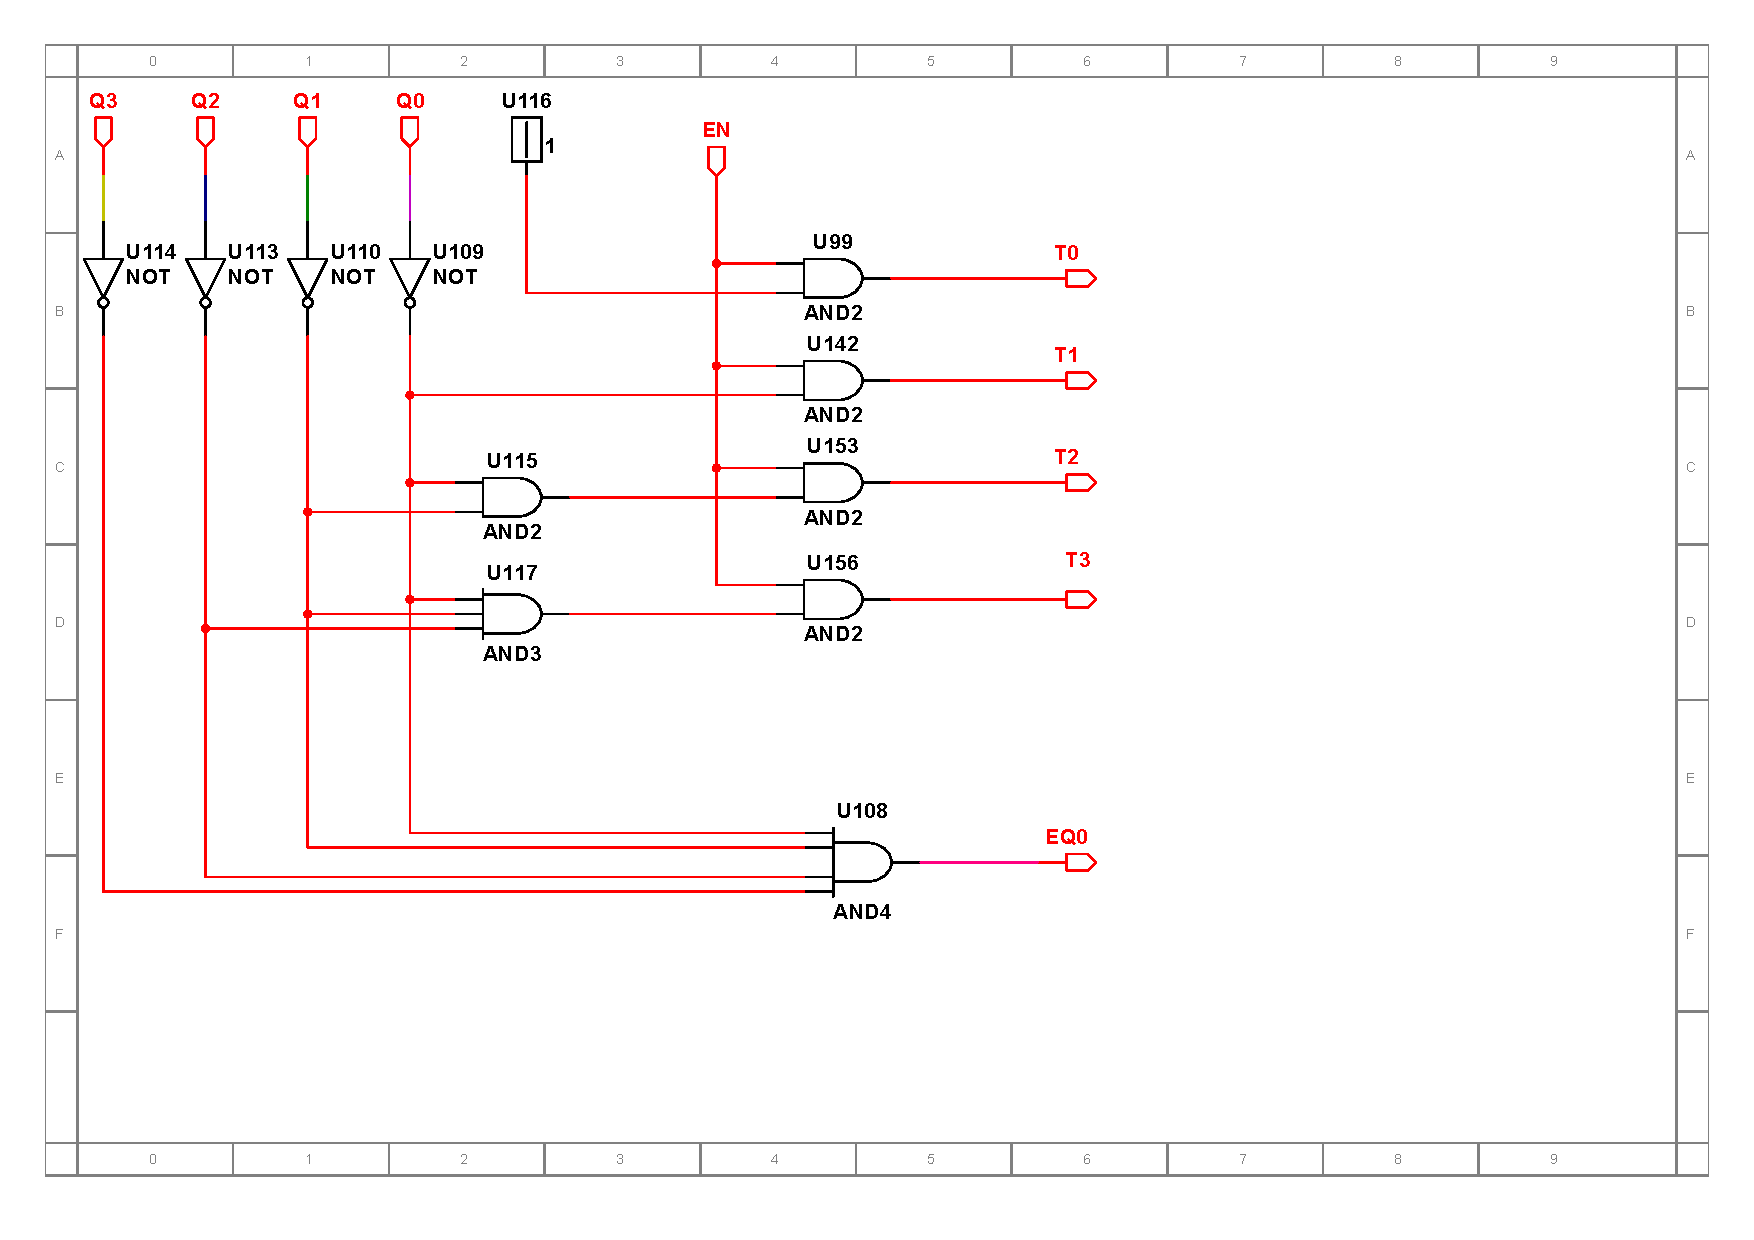
\includegraphics[width=\textwidth]{timer_driver.pdf}
    \captionof{figure}{Schemat podukładu: \texttt{timer\_driver}}
\end{figure}

\pagebreak
\section{Przykład implementacji układu w obwodzie}
Zestawiliśmy przykładowy układ prezentujący jak zaimplementować układ w obwodzie. Użyliśmy
transkodera BCD który zaprojektowaliśmy podczas pierwszego laboratorium. Przekształca on 
6 bitową liczbę zakodowaną binarnie na dwie 4 bitowe liczby binarne będące cyframi wejściowej liczby.

\begin{figure}[H]
    \centering
    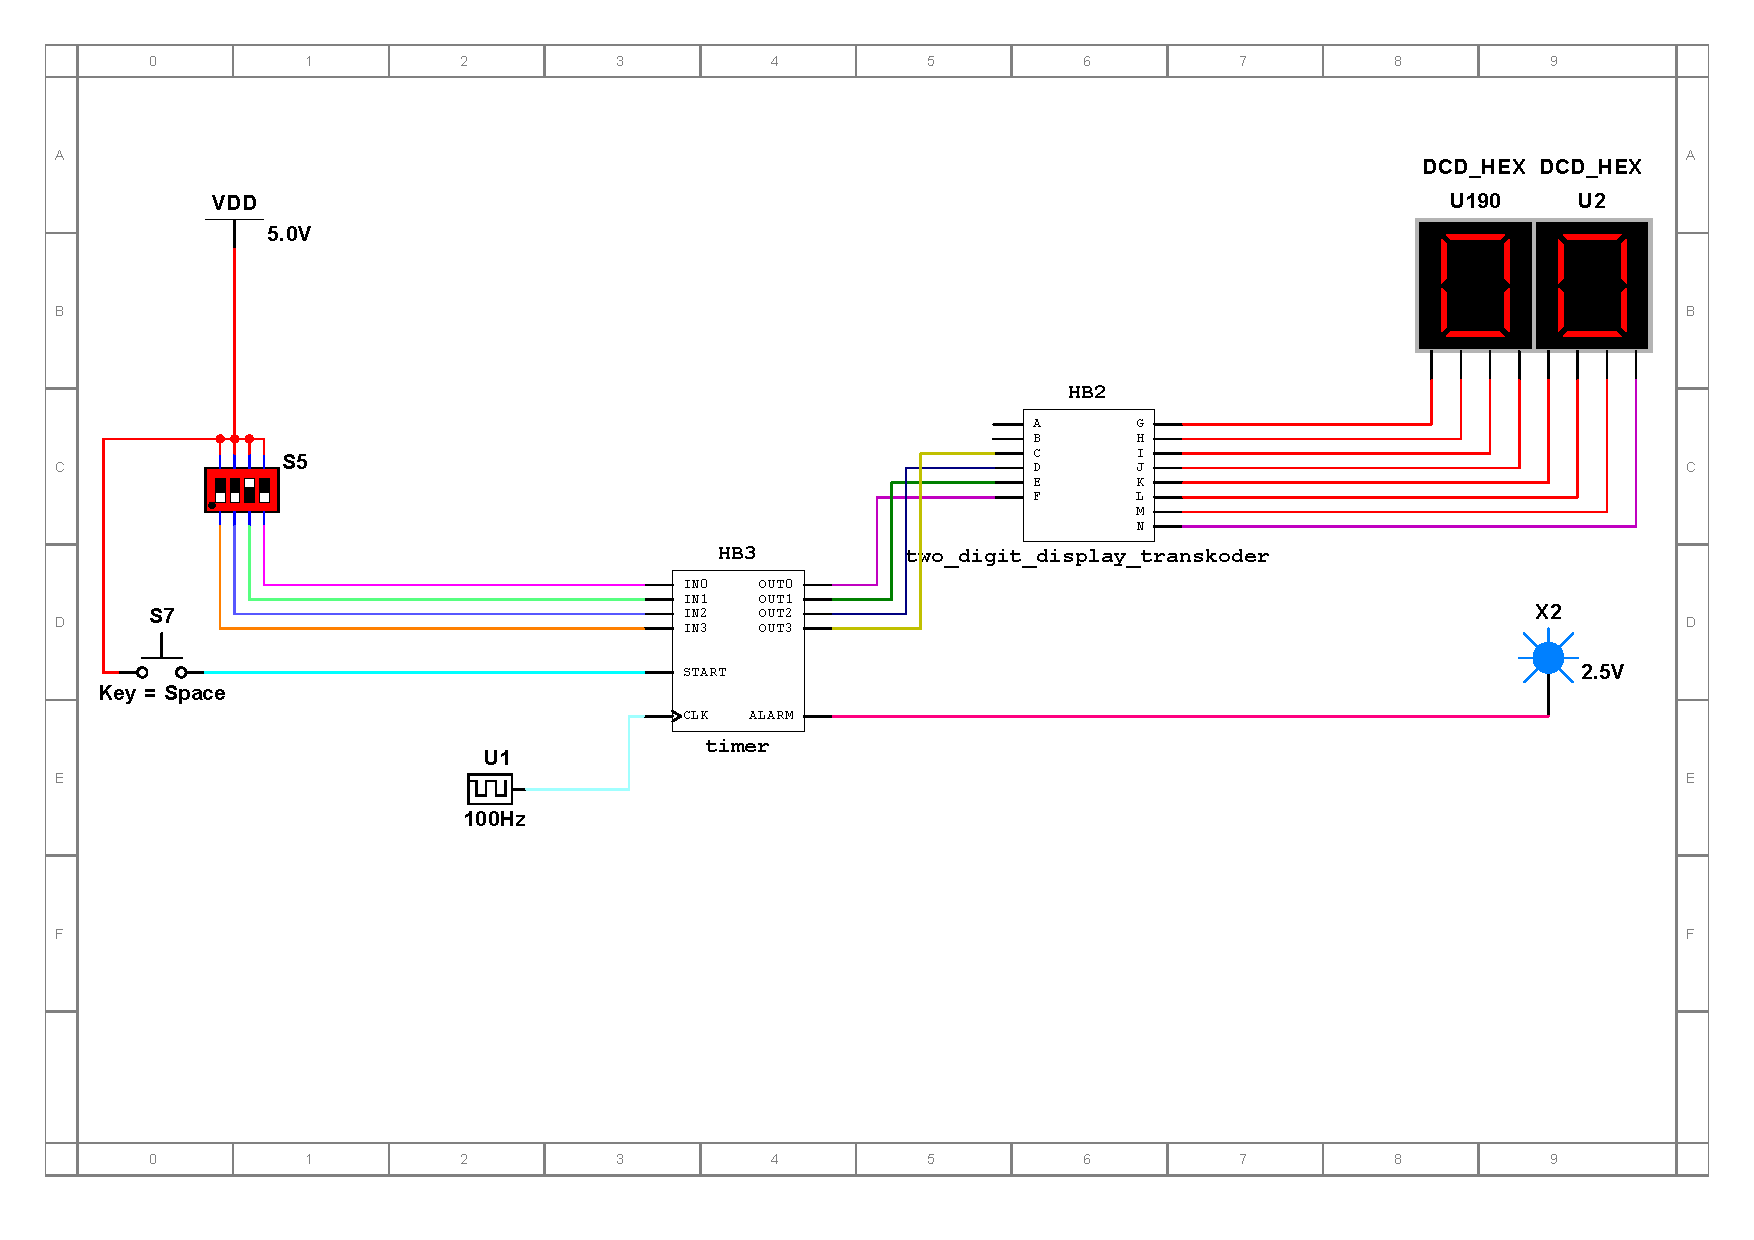
\includegraphics[width=\textwidth]{showup_scheme.pdf}
    \captionof{figure}{Przykładowa implementacja obwodu z wykorzystaniem układu \texttt{timer}}
\end{figure}


\pagebreak
\section{Testy}
\subsection{Testy podukładów}
\subsubsection{Testy timer\_driver}
Aby przetestować układ \verb|timer_driver| użyliśmy układu z generatorem słów, który nadaje dane testowe,
komparatorem do wykrywania błędów, analizatorami stanów logicznych do przedstawienia przebiegu testu i wejść układu oraz
przerzutnikiem JK do sygnalizowania, końcowego wyniku testu na podstawie wszystkich.

\begin{figure}[H]
    \centering
    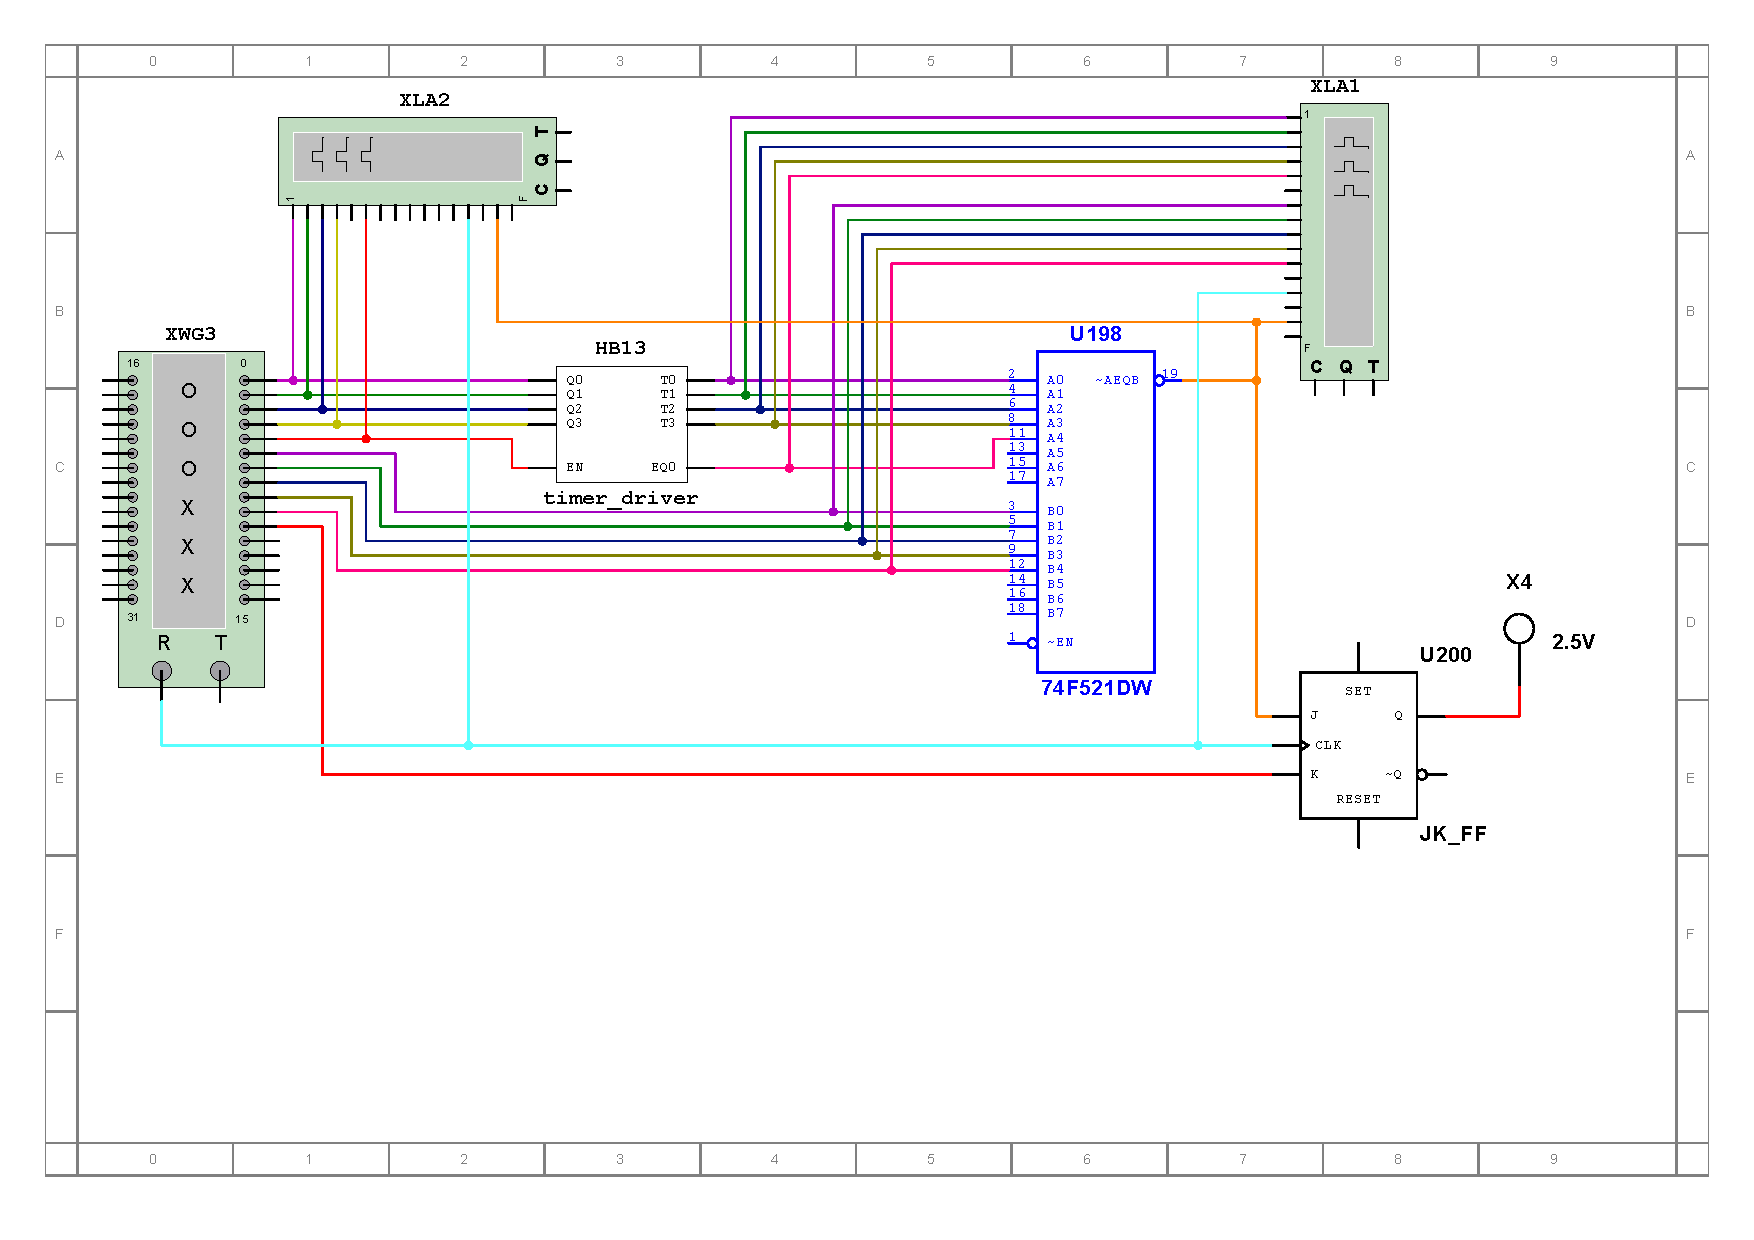
\includegraphics[width=\textwidth]{component_tests_driver.pdf}
    \captionof{figure}{Schemat układu testującego}
\end{figure}

\pagebreak
Aby łatwo wygenerować dane testowe napisaliśmy skrypt w języku python, który generuje 
każdą możliwość danych testowych oraz poprawny dla nich wynik. Kod skryptu:

\small
\begin{minted}[
    frame=lines,
    framesep=2mm,
    baselinestretch=1.2,
    bgcolor=LightGray,
    fontsize=\footnotesize,
    linenos
]{python}
    f = open("driver_test_data.dp", "w")
    f.write("Data:\n")

    ###############################################################################
    # |SR_RESET|EQ0|T3|T2|T1|T0|EN|Q3|Q2|Q1|Q0| #
    ###############################################################################

    class TestOutput: 
        def __init__(self):
            self.in_data = 0
            self.en = 0
            self.output_data = 0
            self.eq0 = 0
            self.reset_sr = 0

        def to_bin_string(self):
            input_binary = str(bin(self.in_data)).removeprefix("0b").rjust(4, '0')
            en_binary = str(bin(self.en)).removeprefix("0b")
            output_binary = str(bin(self.output_data)).removeprefix("0b").rjust(4, '0')
            eq0_binary = str(bin(self.eq0)).removeprefix("0b")
            reset_sr_binary = str(bin(self.reset_sr)).removeprefix("0b")

            return reset_sr_binary + eq0_binary + output_binary + en_binary + input_binary
        

        def to_hex_string(self, pad):
            hex_val = hex(int(self.to_bin_string(), 2))
            return hex_val.removeprefix("0x").rjust(pad, '0')


    ####################################
    # Test cycle to reset JK flip flop #
    ####################################

    reset_to = TestOutput()
    reset_to.eq0 = 1
    reset_to.reset_sr = 1
    f.write(reset_to.to_hex_string(8) + "\n")
    f.write(reset_to.to_hex_string(8) + "\n")
    reset_to.reset_sr = 0
    f.write(reset_to.to_hex_string(8) + "\n")
    data_count = 3

    to = TestOutput()
    for input in range(15, -1, -1):
        to.in_data = input
        to.eq0 = 1 if input == 0 else 0

        f.write(to.to_hex_string(8) + "\n")
        data_count += 1

    to.en = 1
    for input in range(15, -1, -1):
        to.in_data = input
        to.output_data = input ^ 15 if input == 0 else input ^ (input - 1)
        to.eq0 = 1 if input == 0 else 0

        f.write(to.to_hex_string(8) + "\n")
        data_count += 1


    f.write("Initial:\n")
    f.write("0000\n")
    f.write("Final:\n")
    f.write(str(hex(data_count)).capitalize().removeprefix("0x").rjust(4, '0'))

    f.close()
\end{minted}
\captionof{figure}{Skrypt generujący dane do testów, napisany w języku Python}
\Large

Po zaimportowaniu pliku, który wygenerował skrypt generator słów przedstawia się następująco:
\begin{figure}[H]
    \centering

    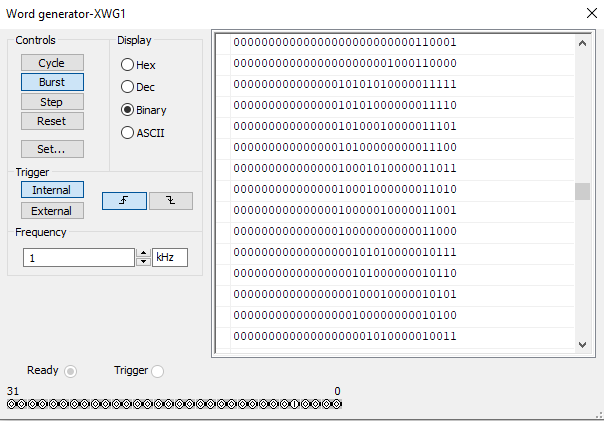
\includegraphics{driver_test_word_generator.png}
    \caption{Dane zaimportowane do generatora słów}
\end{figure}
\pagebreak
Poniżej wynik testu w postaci przebiegu analizatorów stanów logicznych:
\begin{figure}[H]
    \centering
    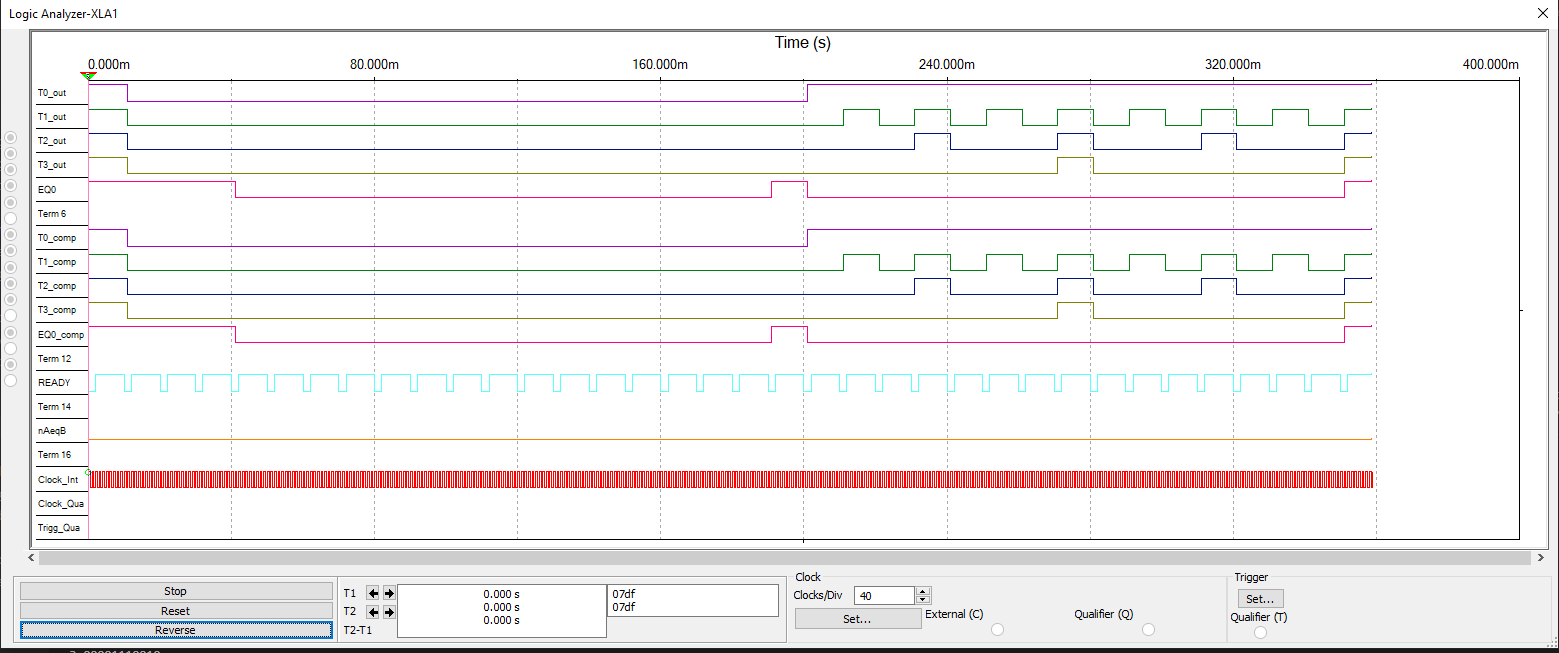
\includegraphics[width=\textwidth]{component_test_logic_analyzer_xla1_driver.png}
    \captionof{figure}{Przebieg sygnałów w analizatorze stanów logicznych podpiętym do wyjścia układu}
\end{figure}
\begin{figure}[H]
    \centering
    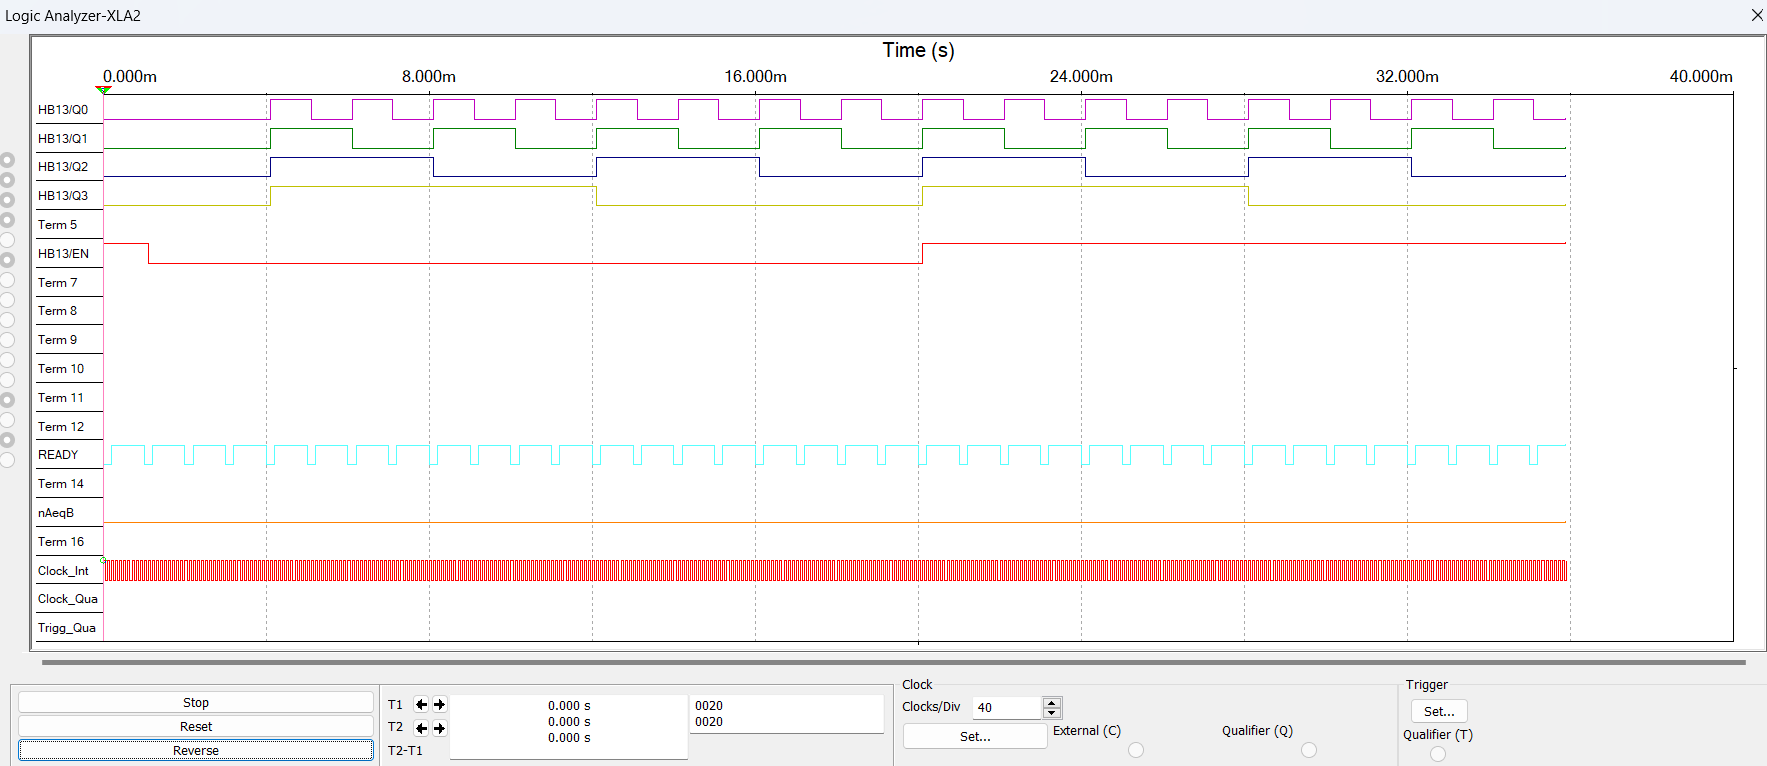
\includegraphics[width=\textwidth]{component_test_logic_analyzer_xla2_driver.png}
    \captionof{figure}{Przebieg sygnałów w analizatorze stanów logicznych podiętego do wejścia układu}
\end{figure}
\pagebreak
\subsubsection{Testy timer\_setter}
Układ dla testów układu \verb|timer_setter| jest podobny do poprzedniego układu tylko z różnicą, że
z powodu ilości wyjść i wejść musieliśmy użyć dwóch analizatorów stanów logicznych do śledzenia przebiegu testu - ich wynik 
można zsynchronizować na podstawie przebiegu sygnału READY oraz czasu rozpoczęcia i zakończenia testu.
Dodaliśmy również trzeci analizator w celu przedstawia wejść testowanego układu.

\begin{figure}[H]
    \centering
    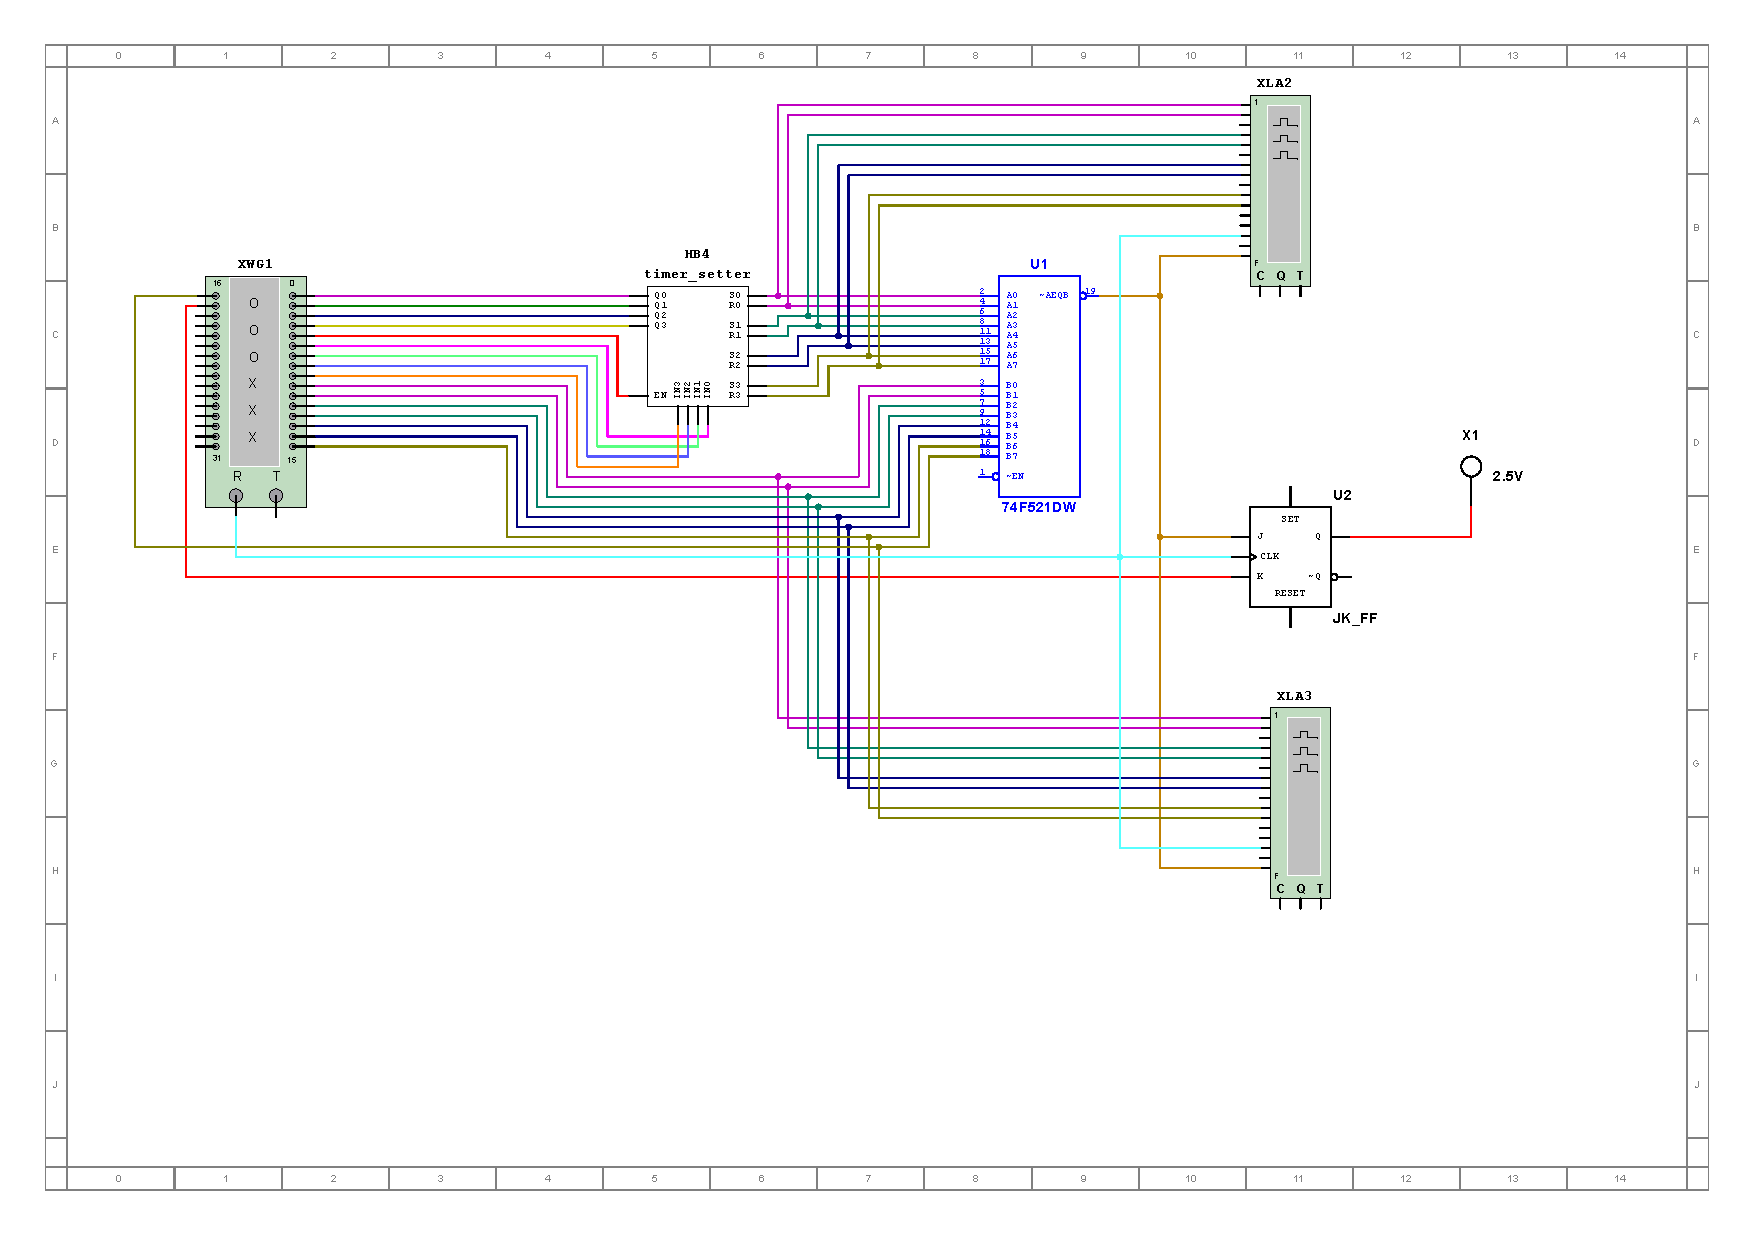
\includegraphics[width=\textwidth]{component_tests_setter.pdf}
    \captionof{figure}{Schemat układu testującego}
\end{figure}
\pagebreak
Podobnie jak wcześniej napisaliśmy skrypt generujący dane:
\small
\begin{minted}[
    frame=lines,
    framesep=2mm,
    baselinestretch=1.2,
    bgcolor=LightGray,
    fontsize=\footnotesize,
    linenos
]{python}
    f = open("setter_test_data.dp", "w")
    f.write("Data:\n")

    ###############################################################################
    # |SR_RESET|S3|R3|S2|R2|S1|R1|S0|R0|IN3|IN2|IN1|IN0|EN|Q3|Q2|Q1|Q0| #
    ###############################################################################

    class TestOutput: 
        def __init__(self):
            self.q_in_data = 0
            self.en = 0
            self.in_data = 0
            
            self.s0 = 0
            self.r0 = 0
            self.s1 = 0
            self.r1 = 0
            self.s2 = 0
            self.r2 = 0
            self.s3 = 0
            self.r3 = 0

            self.reset_sr = 0

        def to_bin_string(self):
            q_input_binary = str(bin(self.q_in_data)).removeprefix("0b").rjust(4, '0')
            en_binary = str(bin(self.en)).removeprefix("0b")
            input_binary = str(bin(self.in_data)).removeprefix("0b").rjust(4, '0')
            
            s0_binary = str(bin(self.s0)).removeprefix("0b")
            r0_binary = str(bin(self.r0)).removeprefix("0b")
            s1_binary = str(bin(self.s1)).removeprefix("0b")
            r1_binary = str(bin(self.r1)).removeprefix("0b")
            s2_binary = str(bin(self.s2)).removeprefix("0b")
            r2_binary = str(bin(self.r2)).removeprefix("0b")
            s3_binary = str(bin(self.s3)).removeprefix("0b")
            r3_binary = str(bin(self.r3)).removeprefix("0b")
            
            reset_sr_binary = str(bin(self.reset_sr)).removeprefix("0b")

            return (reset_sr_binary + 
                    r3_binary + 
                    s3_binary + 
                    r2_binary + 
                    s2_binary + 
                    r1_binary + 
                    s1_binary + 
                    r0_binary + 
                    s0_binary + 
                    input_binary + 
                    en_binary +
                    q_input_binary)
        

        def to_hex_string(self, pad):
            hex_val = hex(int(self.to_bin_string(), 2))
            return hex_val.removeprefix("0x").rjust(pad, '0')


    ####################################
    # Test cycle to reset JK flip flop #
    ####################################

    reset_to = TestOutput()
    reset_to.reset_sr = 1
    f.write(reset_to.to_hex_string(8) + "\n")
    f.write(reset_to.to_hex_string(8) + "\n")
    reset_to.reset_sr = 0
    f.write(reset_to.to_hex_string(8) + "\n")
    data_count = 3

    to = TestOutput()
    for input in range(15, -1, -1):
        for q_input in range(15, -1, -1):
            to.in_data = input
            to.q_input = q_input
            

            f.write(to.to_hex_string(8) + "\n")
            data_count += 1

    to.en = 1
    for input in range(15, -1, -1):
        for q_input in range(15, -1, -1):
            to.in_data = input
            to.q_in_data = q_input
            
            in_bin = bin(input).removeprefix("0b").rjust(4, '0')
            q_in_bin = bin(q_input).removeprefix("0b").rjust(4, '0')

            to.s0 = 1 if in_bin[3] == "1" and q_in_bin[3] == "0" else 0
            to.r0 = 1 if in_bin[3] == "0" and q_in_bin[3] == "1" else 0

            to.s1 = 1 if in_bin[2] == "1" and q_in_bin[2] == "0" else 0
            to.r1 = 1 if in_bin[2] == "0" and q_in_bin[2] == "1" else 0

            to.s2 = 1 if in_bin[1] == "1" and q_in_bin[1] == "0" else 0
            to.r2 = 1 if in_bin[1] == "0" and q_in_bin[1] == "1" else 0

            to.s3 = 1 if in_bin[0] == "1" and q_in_bin[0] == "0" else 0
            to.r3 = 1 if in_bin[0] == "0" and q_in_bin[0] == "1" else 0

            f.write(to.to_hex_string(8) + "\n")
            data_count += 1


    f.write("Initial:\n")
    f.write("0000\n")
    f.write("Final:\n")
    f.write(str(hex(data_count)).capitalize().removeprefix("0x").rjust(4, '0'))

    f.close()
\end{minted}
\captionof{figure}{Skrypt generujący dane do testów, napisany w języku Python}
\Large

\pagebreak
Po zaimportowaniu pliku, który wygenerował skrypt generator słów przedstawia się następująco:
\begin{figure}[H]
    \centering

    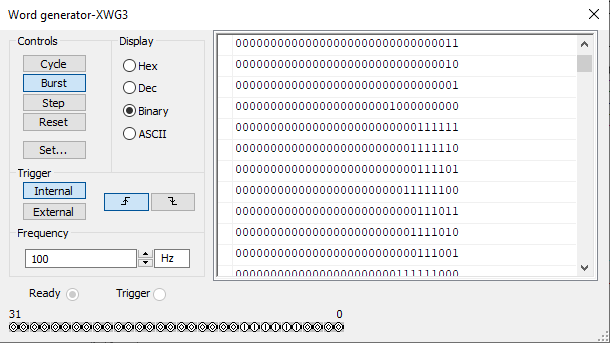
\includegraphics{setter_test_word_generator.png}
    \caption{Dane zaimportowane do generatora słów}
\end{figure}

\pagebreak
Poniżej przebieg wszystkich trzech analizatorów stanów logicznych:
\begin{figure}[H]
    \centering
    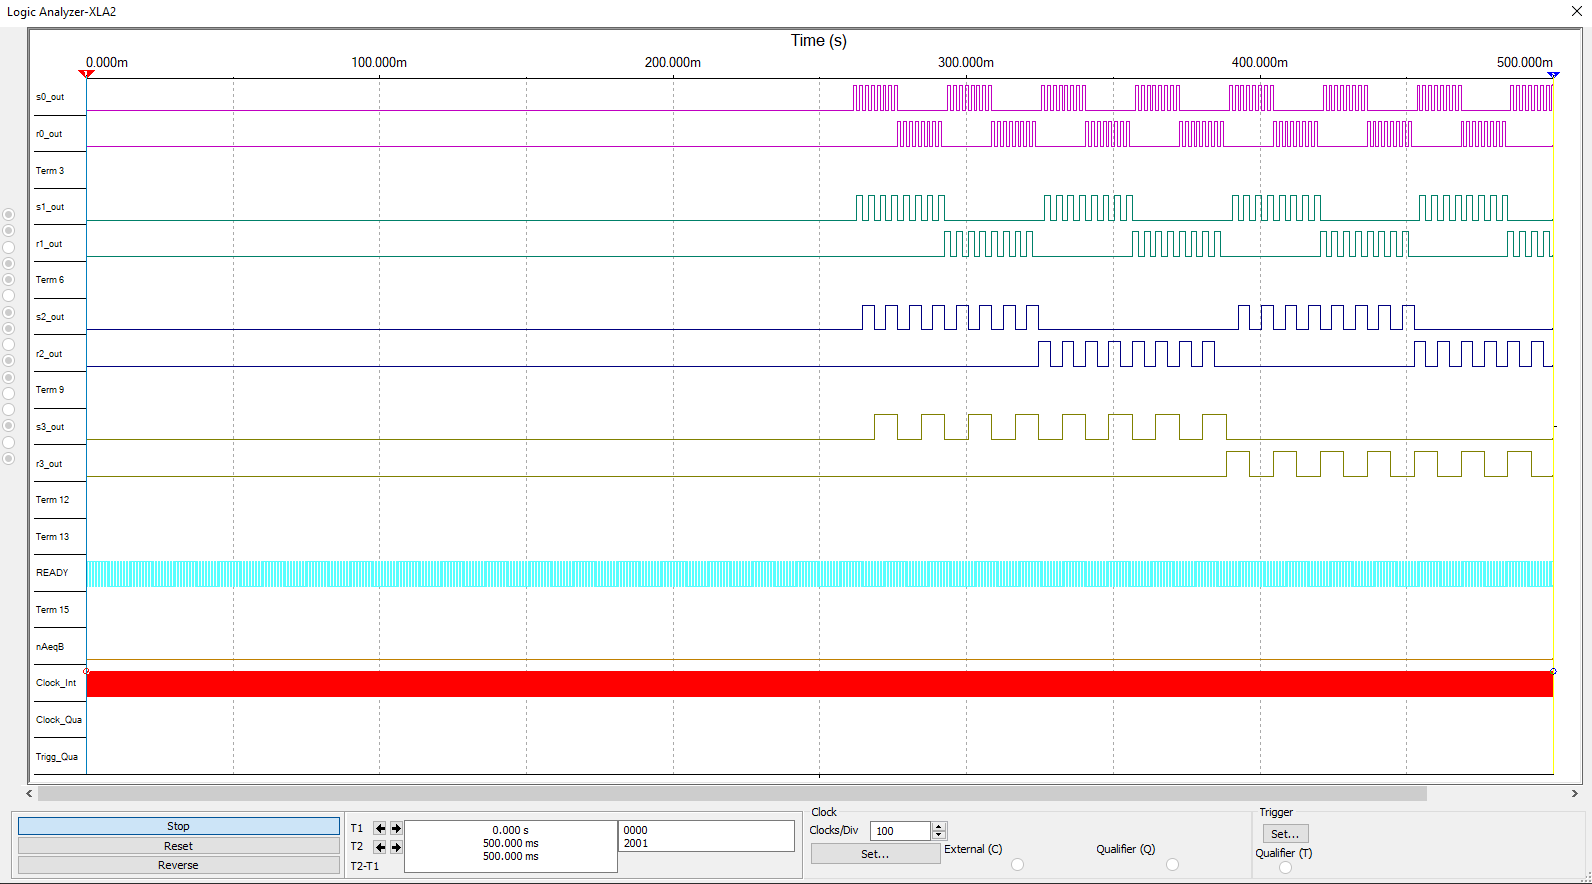
\includegraphics[width=\textwidth]{component_test_logic_analyzer_xla2_setter.png}
    \captionof{figure}{Przebieg sygnałów w analizatorze stanów logicznych podpiętym do wyjścia układu}
\end{figure}

\begin{figure}[H]
    \centering
    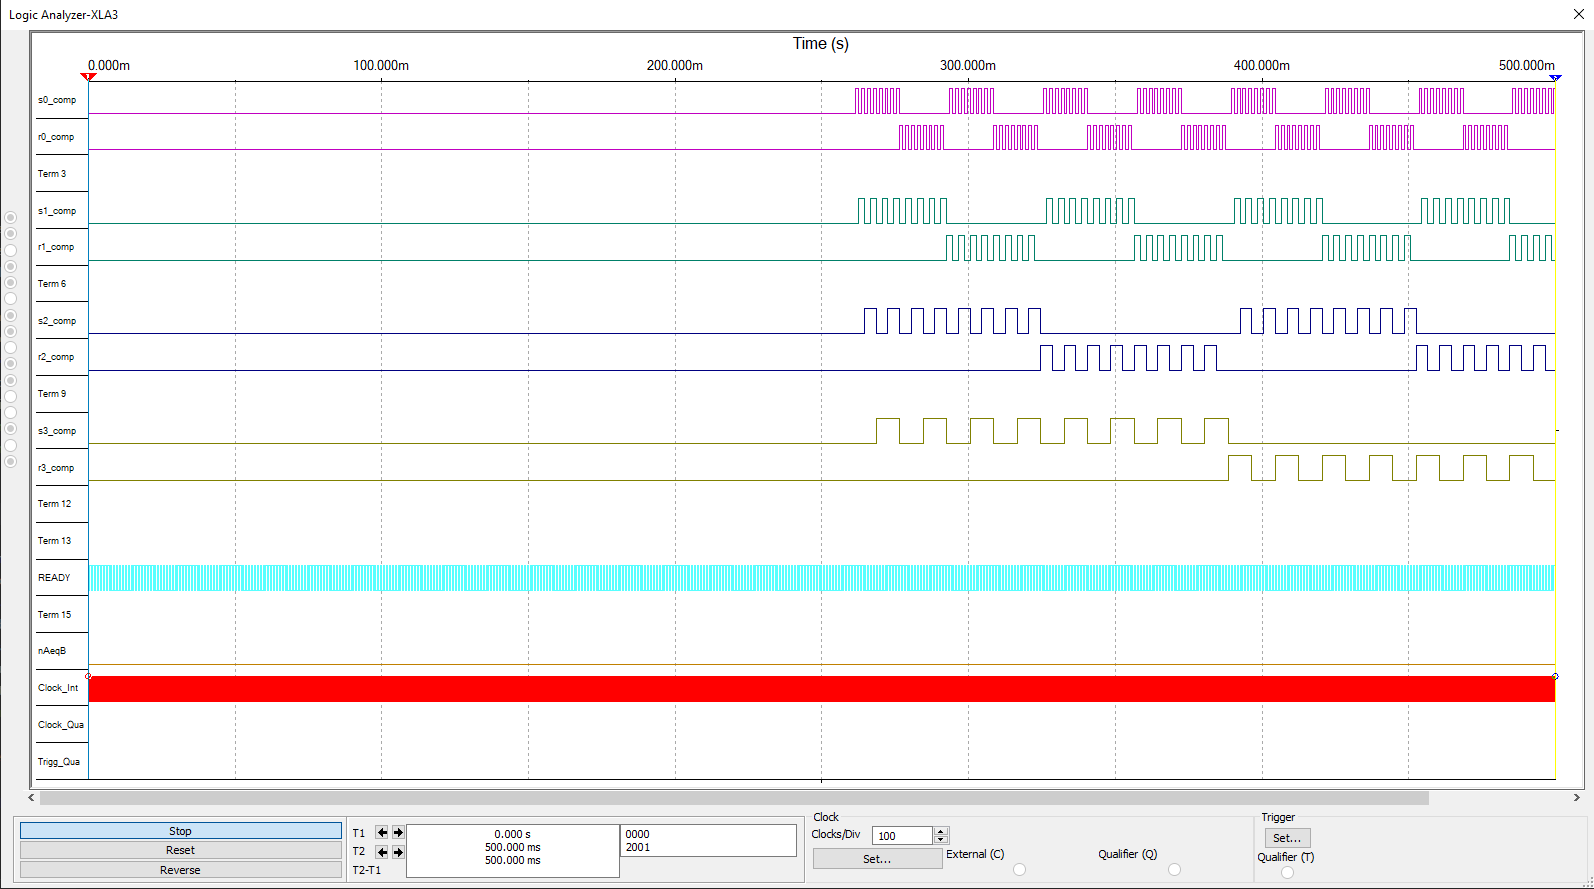
\includegraphics[width=\textwidth]{component_test_logic_analyzer_xla3_setter.png}
    \captionof{figure}{Przebieg sygnałów w analizatorze stanów logicznych podpiętym do wyjścia danych porównawczych}
\end{figure}

\begin{figure}[H]
    \centering
    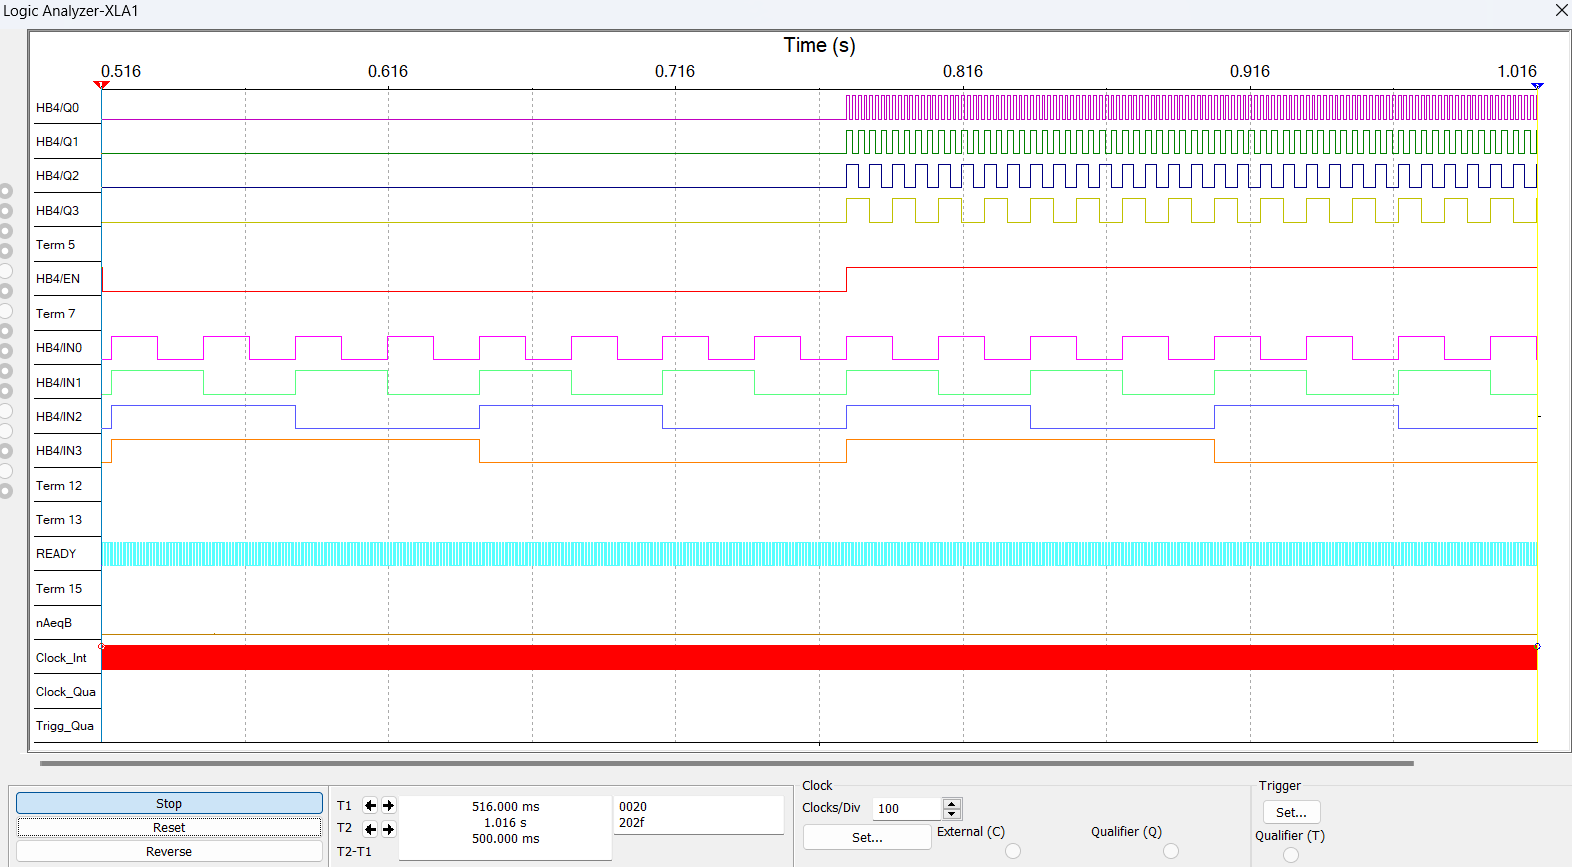
\includegraphics[width=\textwidth]{component_test_logic_analyzer_xla1_setter.png}
    \captionof{figure}{Przebieg sygnałów w analizatorze stanów logicznych podpiętym do wejścia układu}
\end{figure}

\pagebreak
\subsection{Test timera}
Zdecydowaliśmy się przeprowadzić ogólny test układu timer - na najwyższym poziomie abstrakcji.
W tym celu zestawiliśmy układ składający się z generatora słów, naszego układu \verb|timer|, komparatora oraz analizatora
stanów logicznych. Generator słów obsługuje nasz timer zapewniając mu cykle zegara w kolejnych 
generowanych słowach oraz generujący dane porównawcze dla każdego cyklu.

\begin{figure}[H]
    \centering
    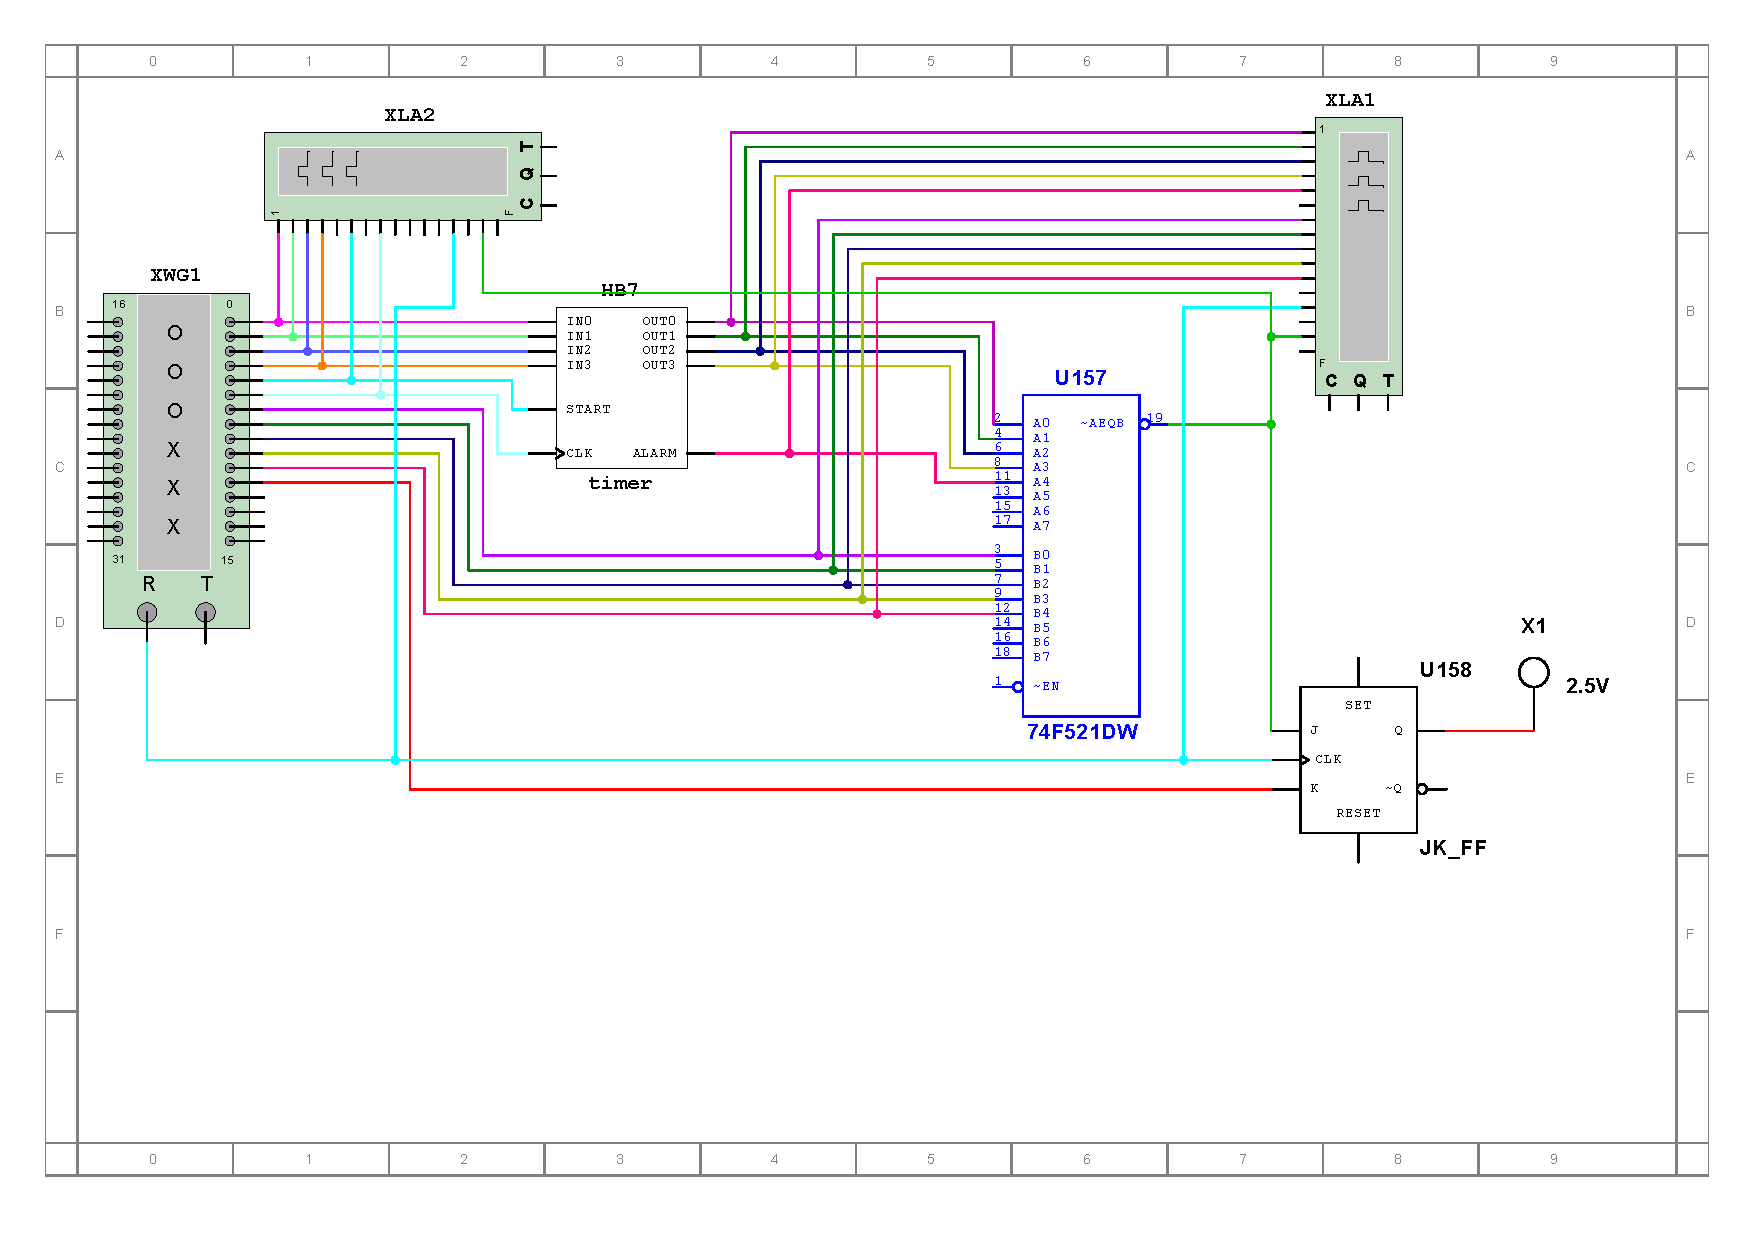
\includegraphics[width=\textwidth]{general_test.pdf}
    \captionof{figure}{Schemat układu testującego}
\end{figure}

Zastosowaliśmy przerzutnik JK próbkujący wyjście komparatora, gdy generator słów generuje wyjście R(READY)
oznaczające, że skończył on generować dane słowo. Pojawienie się stanu wysokiego na wejściu J przerzutnika JK
powoduje jego ustawienie, a pojawienie się stanu wysokiego na wyjściu K resetuje ten przerzutnik.

Do wygenerowanie pliku wejściowego dla generatora słów, napisaliśmy skrypt w języku python, który 
symuluje kolejne kroki odliczania timera w zmiennych i zapisuje je do pliku w formacie, który można zaimportować 
do multisima.

\pagebreak
Poniżej kod skryptu generującego dane:
\small
\begin{minted}[
    frame=lines,
    framesep=2mm,
    baselinestretch=1.2,
    bgcolor=LightGray,
    fontsize=\footnotesize,
    linenos
]{python}
f = open("test_data.dp", "w")
f.write("Data:\n")

##################################################################
# |SR_RESET|ALARM|OUT3|OUT2|OUT1|OUT0|CLK|START|IN3|IN2|IN1|IN0| #
##################################################################

class TestOutput: 
    def __init__(self):
        self.in_data = 0
        self.start = 0
        self.clk = 0
        self.output_data = 0
        self.alarm = 0
        self.reset_sr = 0

    def to_bin_string(self):
        input_binary = str(bin(self.in_data)).removeprefix("0b").rjust(4, '0')
        start_binary = str(bin(self.start)).removeprefix("0b")
        clk_binary = str(bin(self.clk)).removeprefix("0b")
        output_binary = str(bin(self.output_data)).removeprefix("0b").rjust(4, '0')
        alarm_binary = str(bin(self.alarm)).removeprefix("0b")
        reset_sr_binary = str(bin(self.reset_sr)).removeprefix("0b")

        return reset_sr_binary + alarm_binary + output_binary + clk_binary + start_binary + input_binary
    

    def to_hex_string(self, pad):
        hex_val = hex(int(self.to_bin_string(), 2))
        return hex_val.removeprefix("0x").rjust(pad, '0')


####################################
# Test cycle to reset JK flip flop #
####################################

reset_to = TestOutput()
reset_to.alarm = 1
reset_to.reset_sr = 1
f.write(reset_to.to_hex_string(8) + "\n")
f.write(reset_to.to_hex_string(8) + "\n")
reset_to.reset_sr = 0
f.write(reset_to.to_hex_string(8) + "\n")
data_count = 3

for i in range(16):
    to = TestOutput()
    to.in_data = i
    to.start = 1
    to.output_data = i 
    to.alarm = int(i == 0)

    f.write(to.to_hex_string(8) + "\n")
    data_count += 1

    to.in_data = 0
    to.start = 0
    to.alarm = int(i == 0)

    for k in range(i):
        to.clk = 1
        to.output_data -= 1
        if to.output_data == 0:
            to.alarm = 1

        f.write(to.to_hex_string(8) + "\n")
        data_count += 1

        to.clk = 0

        f.write(to.to_hex_string(8) + "\n")
        data_count += 1

    f.write(to.to_hex_string(8) + "\n")
    data_count += 1

f.write("Initial:\n")
f.write("0000\n")
f.write("Final:\n")
f.write(str(hex(data_count)).capitalize().removeprefix("0x").rjust(4, '0'))

f.close()
\end{minted}
\captionof{figure}{Skrypt generujący dane do testów, napisany w języku Python}
\Large

% \pagebreak
Po zaimportowaniu danych do generatora słów przedstawia się on następująco:
\begin{figure}[H]
    \centering
    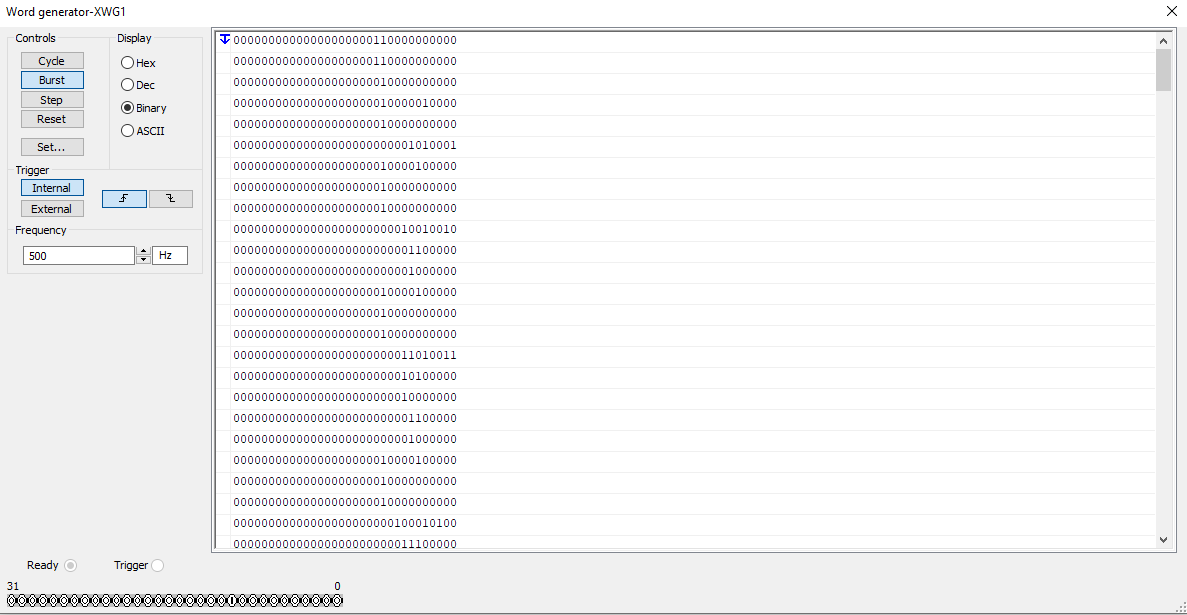
\includegraphics[width=\textwidth]{general_test_word_generator.png}
    \caption{Dane zaimportowane do generatora słów}
\end{figure}

\pagebreak
W wyniku testu otrzymujemy informację poprzez zaświecenie się lampki jeśli gdziekolwiek wystąpił błąd oraz 
przebieg sygnałów z analizatorów stanów logicznych:
\begin{figure}[H]
    \centering
    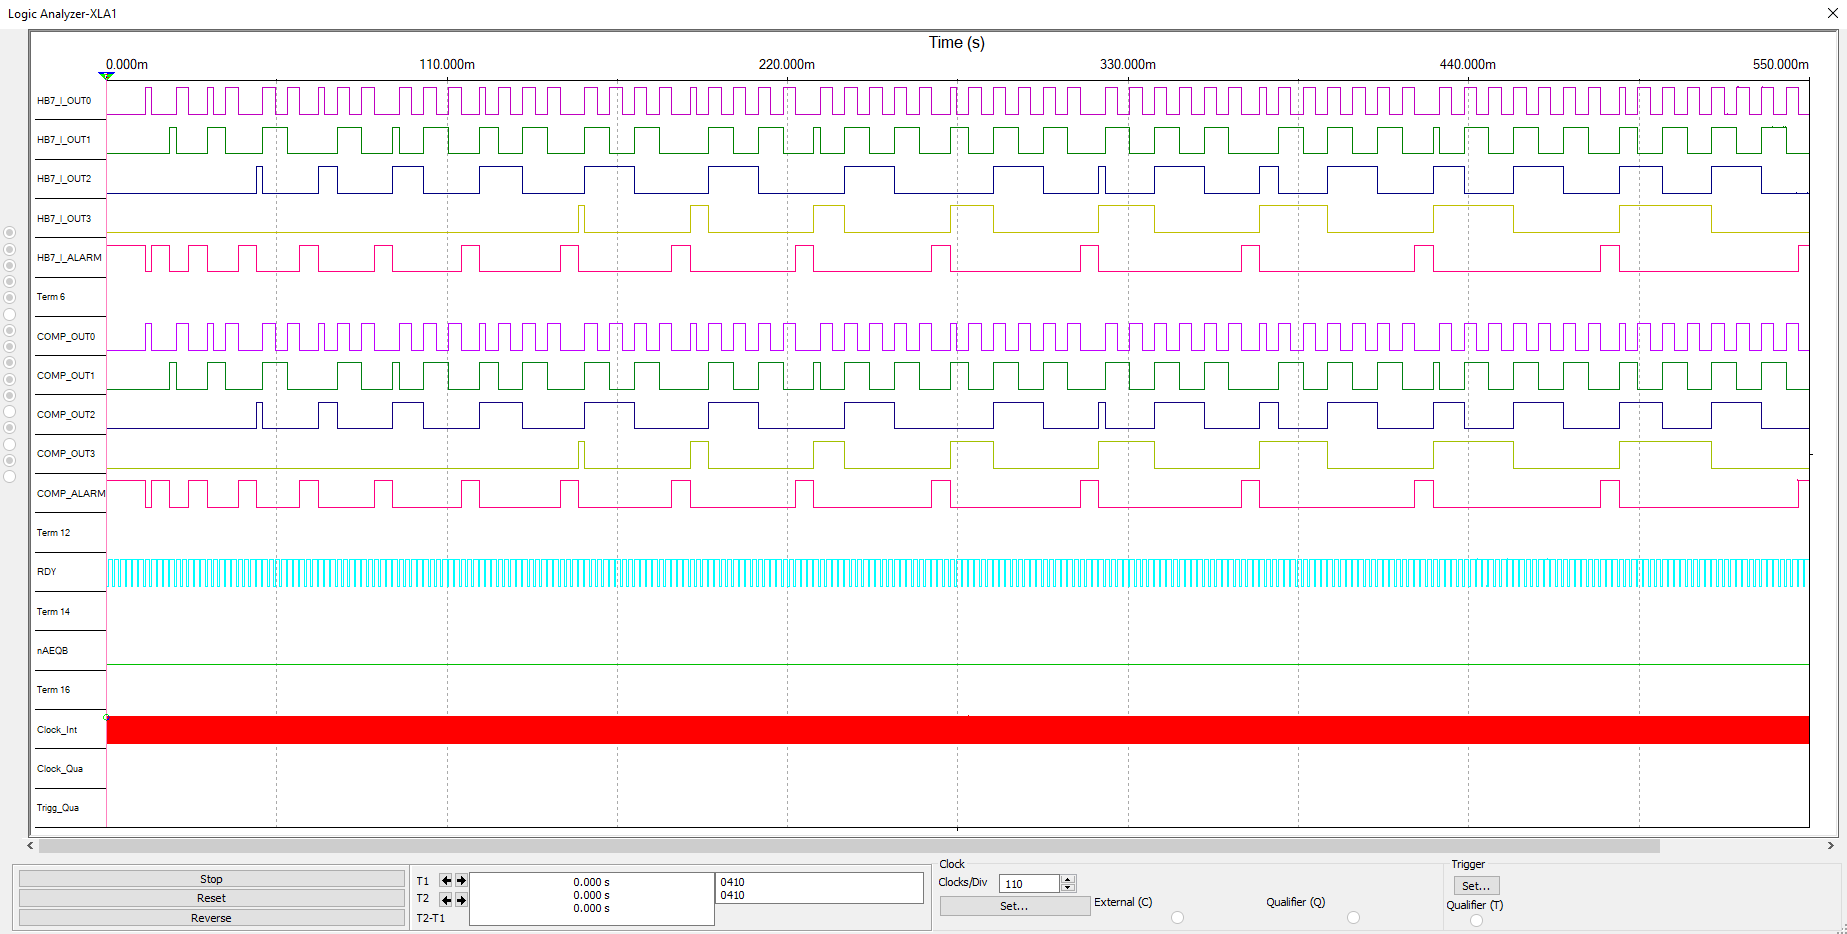
\includegraphics[width=\textwidth]{general_test_logic_analyzer.png}
    \captionof{figure}{Przebieg sygnałów w analizatorze stanów logicznych podpiętym do wyjścia układu}
\end{figure}

\begin{figure}[H]
    \centering
    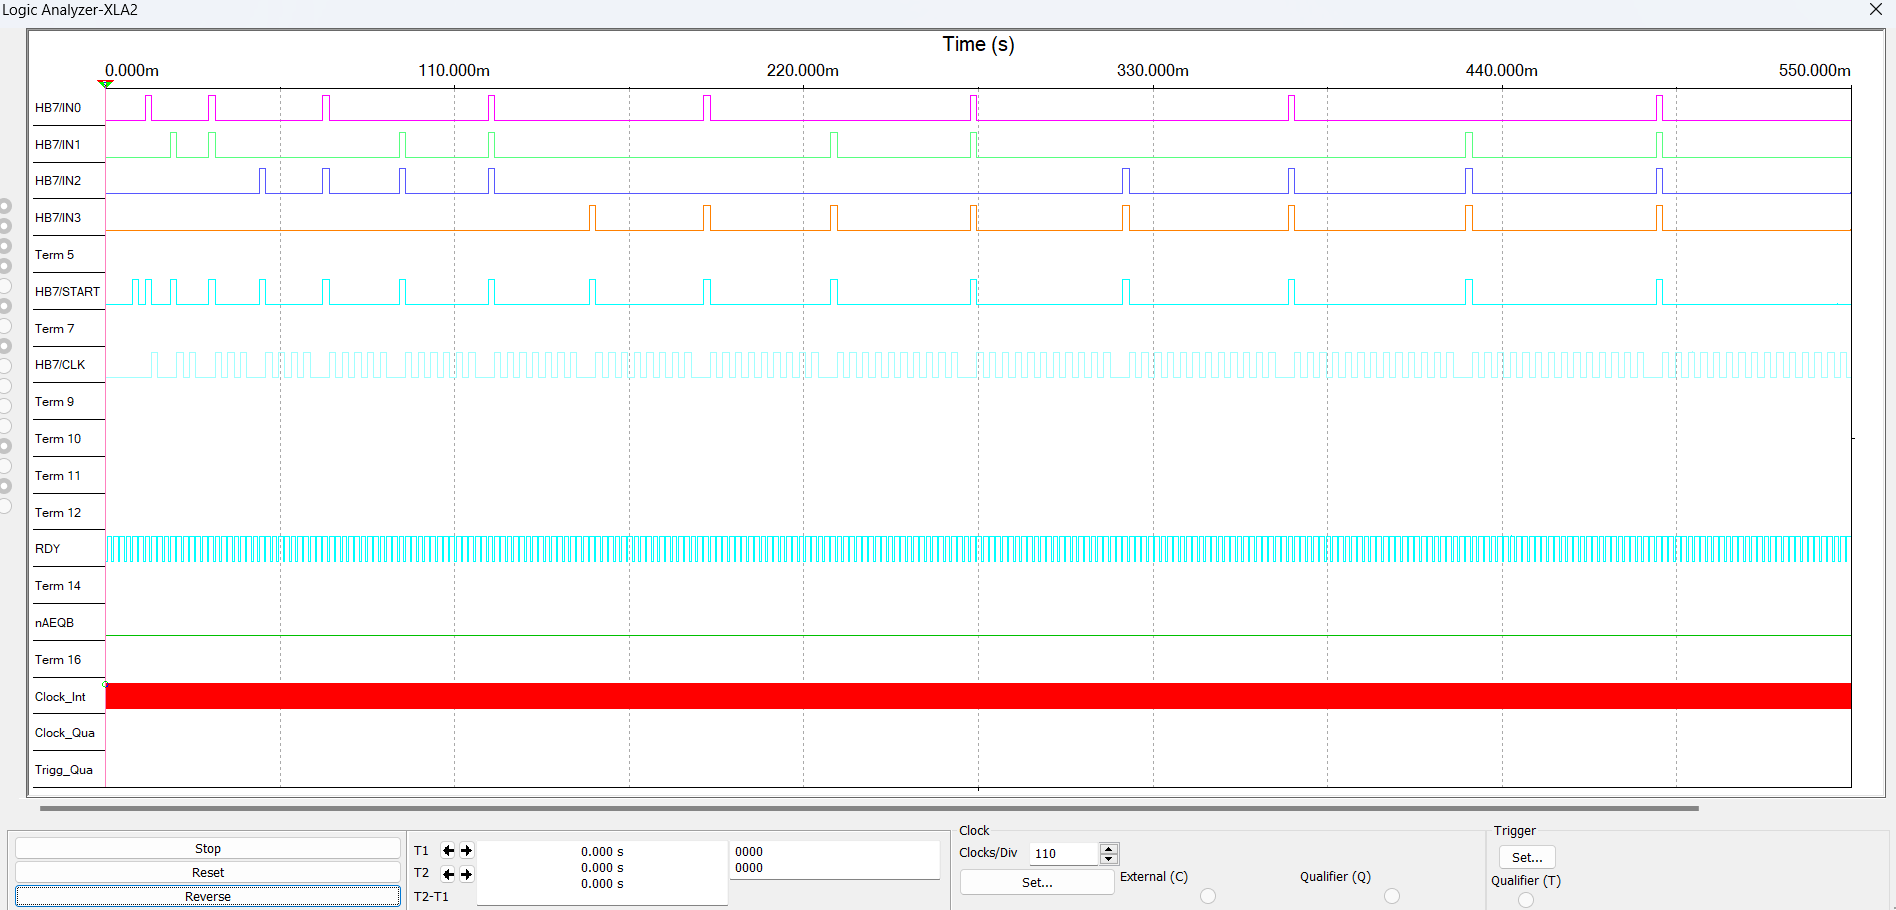
\includegraphics[width=\textwidth]{general_test_logic_analyzer_xla2.png}
    \captionof{figure}{Przebieg sygnałów w analizatorze stanów logicznych podpiętym do wejścia układu}
\end{figure}
\pagebreak
\section{Zastosowania}
\begin{itemize}
    \item Jednym z zastosowań układów timer jest umieszczanie ich w mikroprocesorach. Są one jednym 
            z podstawowych układów peryferyjnych pozwalających na wykonywanie periodycznych 
            zadań. Najbardziej podstawowym zadaniem może być periodyczne wykonywanie specjalnie
            zdefiniowanego fragmentu kodu aktywowanego sygnałem \verb|ALARM| - przerwanie sprzętowe.
            W ten sposób nie musimy tracić czasu procesora na kontrolę czasu aby wykonywać kod. 
            Taki mechanizm można też wykorzystać do periodycznej obsługi innych peryferiów jak np.
            przetwornik analogowo-cyfrowy czy kontrolery magistrali komunikacyjnych.
    \begin{figure}[H]
        \centering
        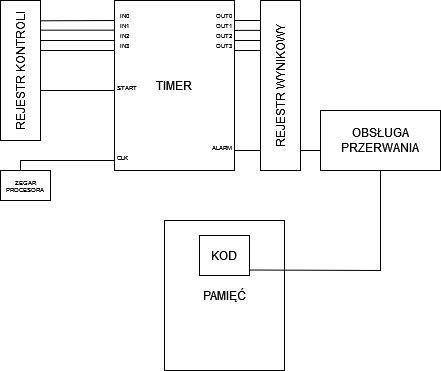
\includegraphics[width=0.7\textwidth]{timer_use_mcu.png}
        \caption{Przykładowe zastosowanie układu timer w mikroprocesorach}
    \end{figure}

    \item W automatycznych systemach nawadniających do roślin,
    odliczający się licznik może być używany do kontrolowania czasu podlewania różnych obszarów ogrodu lub roślin doniczkowych.

    \begin{figure}[H]
        \centering
        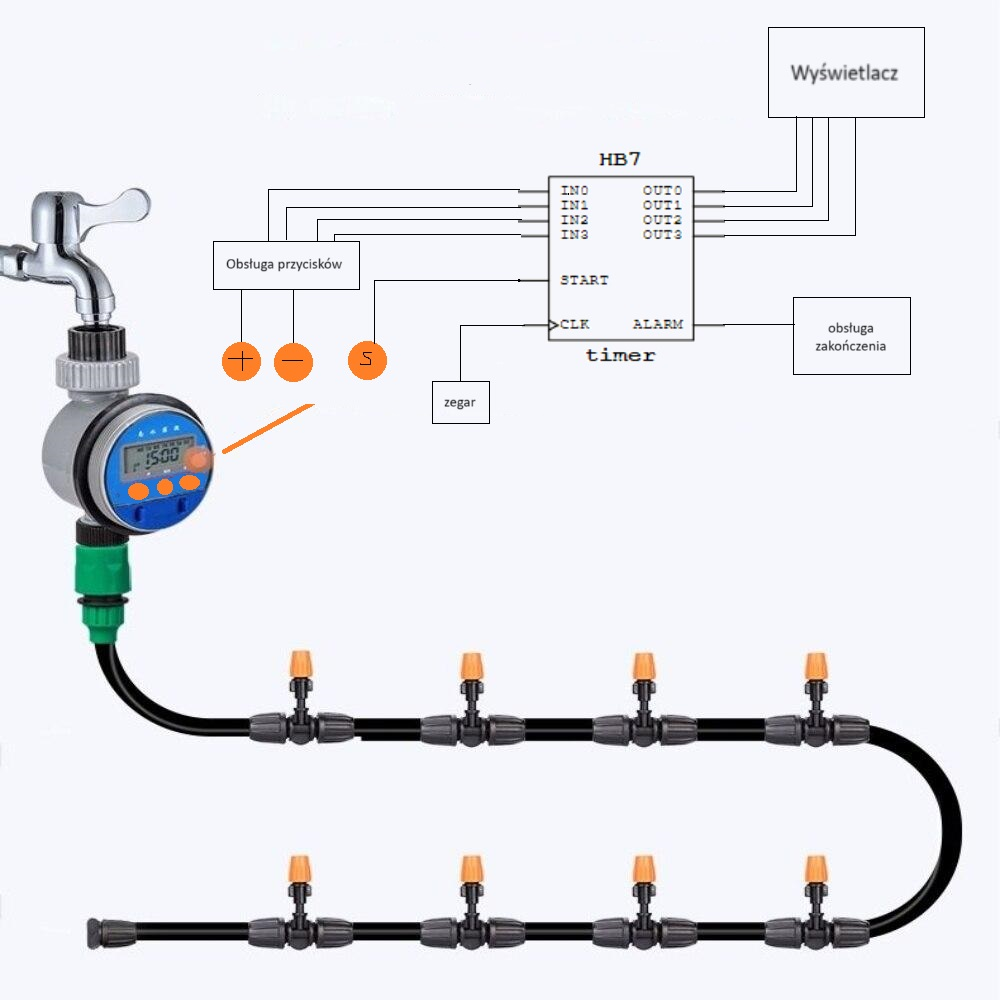
\includegraphics[width=0.7\textwidth]{timer_use2.jpeg}
        \caption{Przykładowe zastosowanie układu timer w systemach nawadniających}
    \end{figure}

    \item Dany układ można również zastosować w lampkach migających, takich jak te używane w alarmach lub sygnalizacji.
    Te lampki mogą zaświecać się cyklicznie co określoną ilość sekund, tworząc efekt migotania lub pulsowania światła.
   Jest to przydatne w przypadku systemów alarmowych, ostrzegawczych lub sygnalizacyjnych. Przykładowo, sygnalizujące awarię sprzętu.

    \item Na liniach produkcyjnych, gdzie maszyny wykonują kolejne etapy produkcji,
     odliczający się licznik może być użyty do synchronizacji czasu między różnymi maszynami.
      Na przykład, jeśli jedna maszyna wykonuje proces przygotowawczy,
       a następnie musi odczekać przed przekazaniem części do kolejnej maszyny.




\end{itemize}

\pagebreak
\section{Wnioski}
Dzięki przerzutnikom możemy projektować złożone układy z pamięcią swojego stanu. 

W toku rozwiązywania postawionego problemu opracowaliśmy kilka możliwych rozwiązań. Ostatecznie
zdecydowaliśmy się na przedstawienie tego konkretnego rozwiązania ze względu na jego prostotę i 
największą niezawodność. Zastosowanie przerzutników działających synchronicznie pozwoliło na zredukowanie
ilości hazardów przy odliczaniu czasu.

Pierwotnym pomysłem było użycie przerzutników T asynchronicznie - łącząc je w szeregowo dzięki czemu 
nie było konieczne projektowanie układu kontrolującego przerzutniki. Największą wadą tego rozwiązania
było to, że otoczka sterowania tak połączonych przerzutników była trudna do przedstawienia wzorami i 
uzasadnienia w prosty sposób. Rozwiązanie opierało się na idei generowania kolejnych impulsów 
synchronizujących kolejne etapy przygotowania i uruchomienia układu.

\begin{figure}[H]
    \centering
    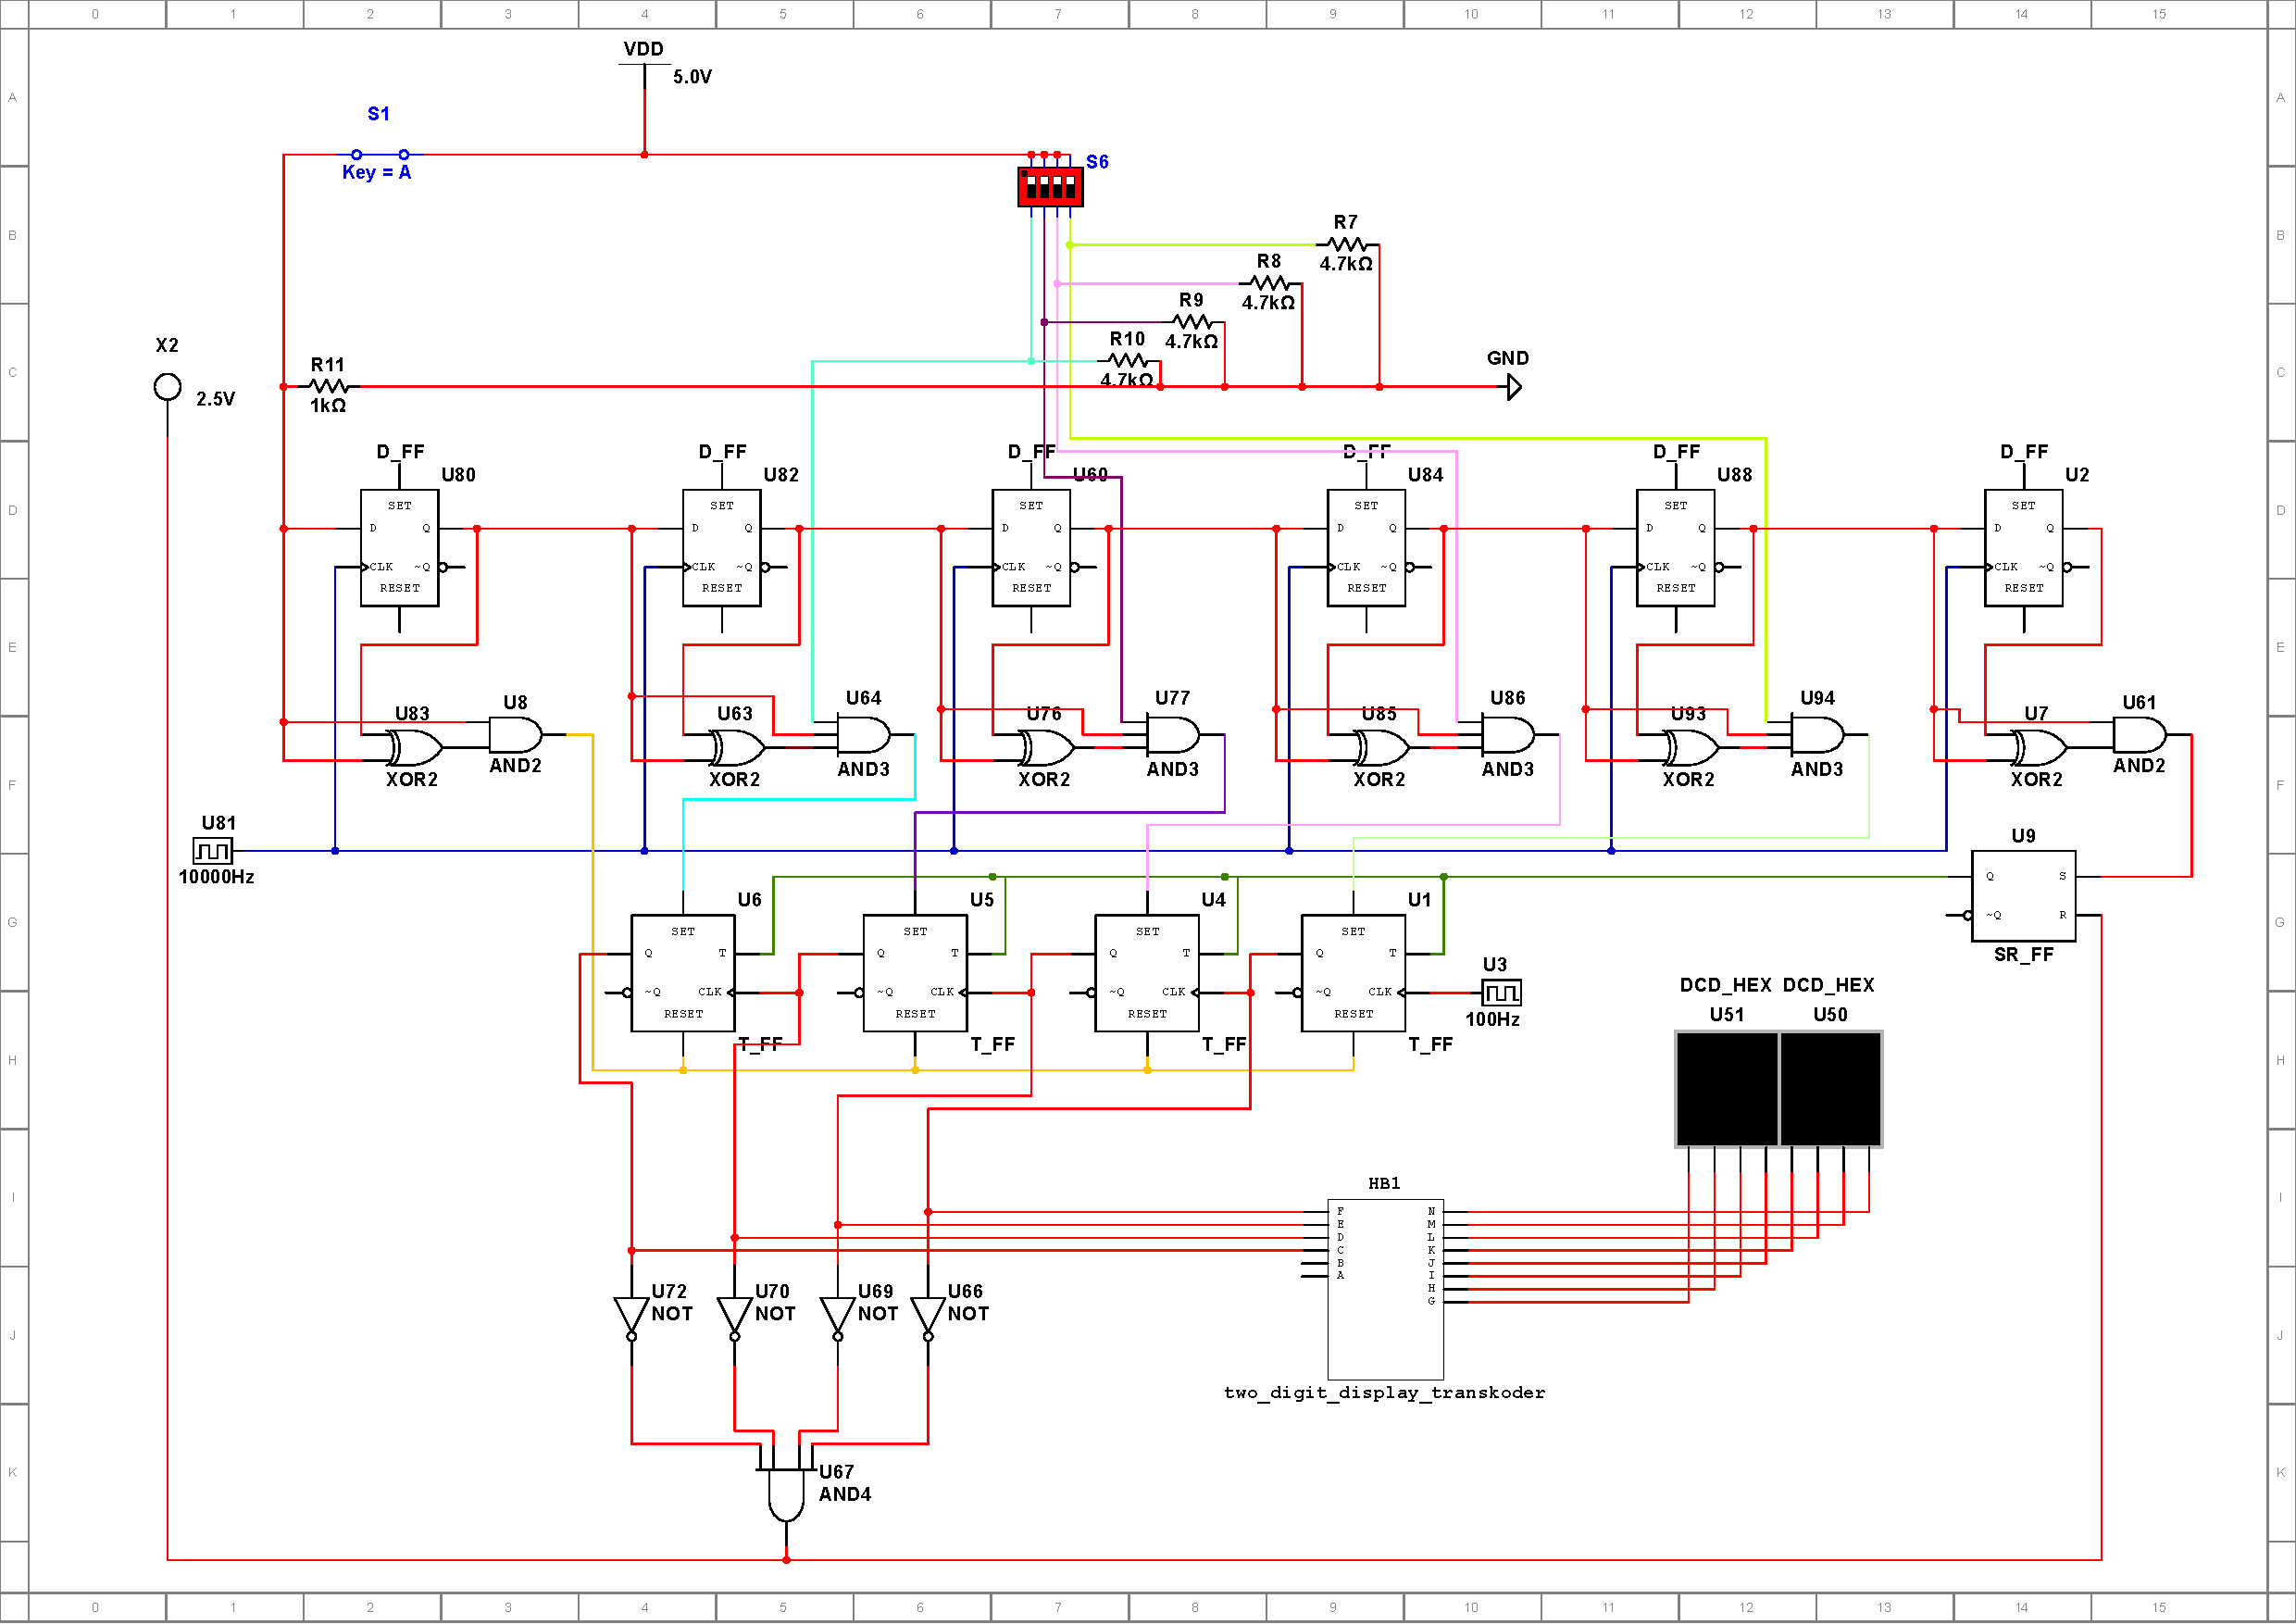
\includegraphics[width=\textwidth]{lab2_1.pdf}
    \captionof{figure}{Schemat pierwszego rozwiązania}
\end{figure}
\pagebreak

Kolejne rozwiązanie opierało się na wykorzystaniu przerzutników JK do zrobienia synchronicznego licznika.
W tym układzie, czas był ustawiany bezpośrednio na przerzutnikach za pomocą przycisków (+) i (-). Było to możliwe
dzięki zaimplementowaniu licznika w sposób pozwalający na jego odliczanie zarówno do przodu jak i do tyłu.
Po wciśnięciu przycisku "start" wybrany czas zostawał zapisywany w rejestrze o równoległych wejściach i wyjściach (PIPO),
a licznik zaczynał odmierzać czas. Po dojściu licznika do zera, aktywował się alarm, a po kolejnym naciśnięciu
przycisku "start" wartość zapisana w rejestrze była wczytywana na licznik i odliczanie zaczynało się od początku.
Ostatecznie zrezygnowaliśmy z tego rozwiązania, ponieważ było ono skomplikowane i pełne trudnych do rozwiązania błędów.
Przede wszystkim jednak, znacznie odbiegało ono od wymogów zadania. Z tych właśnie powodów sama implementacja nigdy
nie została całkowicie dokończona i na schemacie przedstawionym poniżej występują liczne błędy i niedociągnięcia. 

\begin{figure}[H]
    \centering
    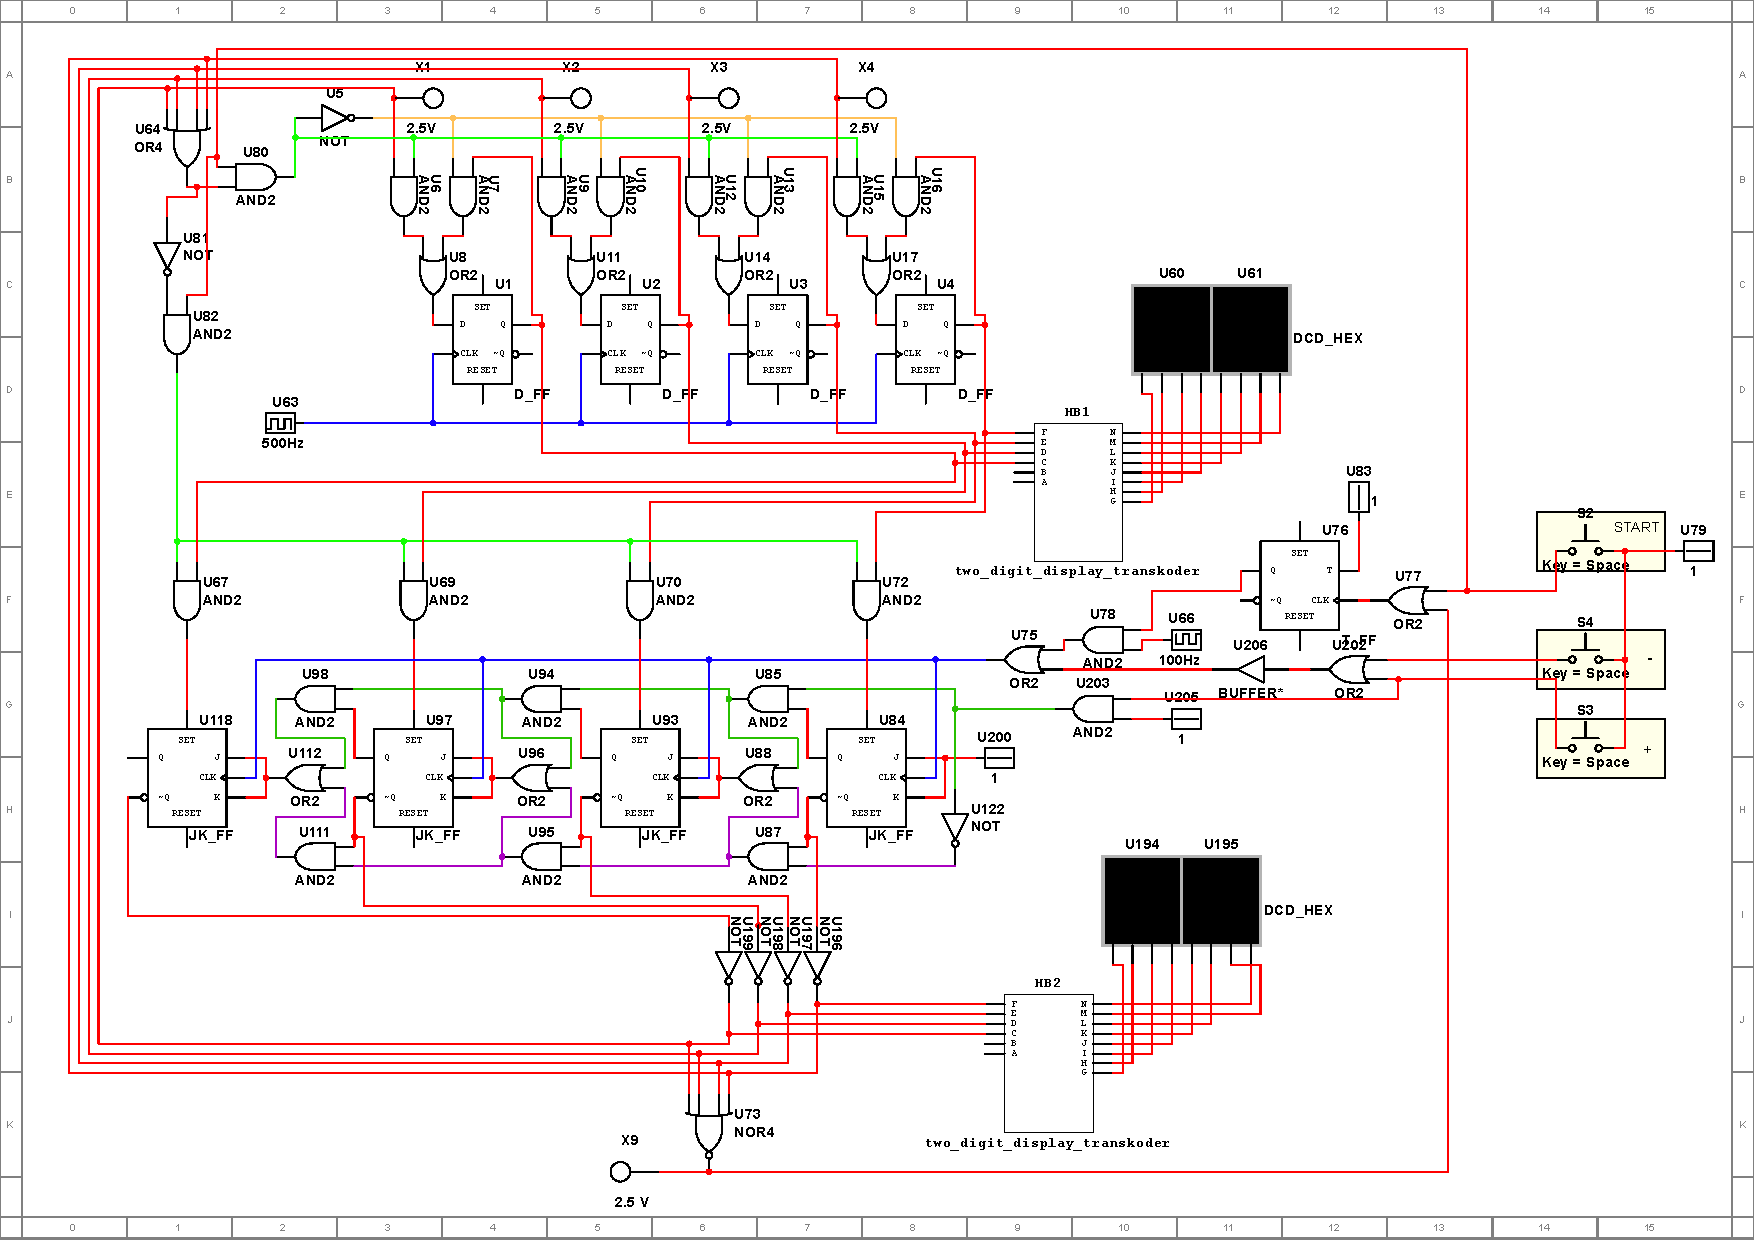
\includegraphics[width=\textwidth]{lab2-alt.pdf}
    \captionof{figure}{Scheamt drugiego rozwiązania}
\end{figure}

\end{document}


